\documentclass[onecolumn, a4paper, 11pt, titlepage]{report}
\renewcommand{\baselinestretch}{1.2} 
\bibliographystyle{IEEEtran}
\usepackage[none]{hyphenat}
\usepackage{a4wide}
\usepackage{float}
\usepackage{multicol}
\usepackage{multirow}
\usepackage{lscape}

\usepackage{amsmath}
\numberwithin{figure}{section}
\usepackage[nottoc,numbib]{tocbibind}
\makeatletter
 \renewcommand*\l@table{\@dottedtocline{3}{2em}{4.5em}}
\makeatother
% \makeatletter
% \@addtoreset{table}{section}
% \makeatother
% \renewcommand\thetable{\arabic{\thesection}-\arabic{table}}

\usepackage{color}
\usepackage{soul}  % for highlighting text etc.
\usepackage{graphicx}
\usepackage{caption}
\usepackage{flafter}
\usepackage{placeins}
\usepackage{cite}
%-------------------------------------------------------------------------------

\newcommand{\micro}{\textmu}
\newcommand{\Ohm}{$\Omega$}

\newcommand{\etal}       {\emph{et~al.}}
\newcommand{\ie}         {i.e.}
\newcommand{\bookcite}[2]{\cite{#1}~pg.~#2}
%-------------------------------------------------------------------------------

\newcounter{author}
\renewcommand{\theauthor}{\stepcounter{author}\raisebox{1ex}{\small\fnsymbol{author}}}
%-------------------------------------------------------------------------------

\renewcommand{\today}{%
 \number\day\space%
 \ifcase\month%
  \or January%
  \or February%
  \or March%
  \or April%
  \or May%
  \or June%
  \or July%
  \or August%
  \or September%
  \or October%
  \or November%
  \or December%
 \fi%
 \space\number\year%
}
%-------------------------------------------------------------------------------

\newlength{\TempFigureLength}
%-------------------------------------------------------------------------------

\newenvironment{FigureEnvironment}{
 \begin{figure}[!t]%
 \begin{center}%
}{
 \end{center}%
 \end{figure}%
}
%-------------------------------------------------------------------------------

\def\FigureSize{0.8}

\newcommand{\Figure}[3][scale=\FigureSize]{%
 \begin{FigureEnvironment}%
  \refstepcounter{figure}
  \addcontentsline{lof}{section}{Fig.~\thefigure{}~~~#2}
  \label{fig:#3}%
  \includegraphics[#1]{Figures/#3}\\[1em]%
  \footnotesize
  \settowidth{\TempFigureLength}{Fig.~\thefigure{}.~~{#2}}
  \ifdim \TempFigureLength > 0.95\columnwidth
   \parbox{0.95\columnwidth}{Fig.~\thefigure{}.~~{#2}}%
  \else
   Fig.~\thefigure{}.~~{#2}%
  \fi
 \end{FigureEnvironment}%
}
%-------------------------------------------------------------------------------

\newenvironment{TableEnvironment}{
 \begin{table}[!t]%
 \begin{center}%
}{
 \end{center}%
 \end{table}%
}
%-------------------------------------------------------------------------------

\renewcommand{\thetable}{\Roman{table}}

\newcommand{\Table}[5]{%
 \begin{TableEnvironment}%
  \refstepcounter{table}
  \addcontentsline{lot}{section}{TABLE \thetable{}~~~#1}
  \label{tab:#5}%
  TABLE \thetable{}\\[1ex]
  \settowidth{\TempFigureLength}{\textsc{#1}}
  \ifdim \TempFigureLength > 0.95\columnwidth
   \parbox{0.95\columnwidth}{\textsc{#1}}%
  \else
   \textsc{#1}%
  \fi\\[1em]
  \renewcommand{\arraystretch}{1.2}
  \begin{tabular}{#2}
   \hline
   \hline
    #3\\
   \hline
    #4
   \hline
   \hline
  \end{tabular}
 \end{TableEnvironment}%
}
%-------------------------------------------------------------------------------

\newcommand{\Plot}[2]{
 \begin{FigureEnvironment}%
  \refstepcounter{figure}
  \addcontentsline{lof}{section}{Fig.~\thefigure{}~~~#1}
  \label{fig:#2}%
  \includegraphics[width=0.95\columnwidth]{../../Octave/Prac_1/#2}\\[1em]%
  \footnotesize
  \settowidth{\TempFigureLength}{Fig.~\thefigure{}.~~{#1}}
  \ifdim \TempFigureLength > 0.95\columnwidth
   \parbox{0.95\columnwidth}{Fig.~\thefigure{}.~~{#1}}%
  \else
   Fig.~\thefigure{}.~~{#1}%
  \fi
 \end{FigureEnvironment}%
}
\usepackage{textcomp} %Used in listings for printing upright quotes
\usepackage{listings} %For typesetting source code
\lstloadlanguages{C++, Matlab, Verilog}
%-------------------------------------------------------------------------------

\lstset{%
 frame      = single,%
 basicstyle = \small\ttfamily,%
 basewidth  = 1.3ex,%
 numberstyle=\tiny, %Austin
 numbers=left,%Austin
 stepnumber=1%Austin
% basicstyle = \scriptsize\ttfamily,%
% basewidth  = 1.2ex%
}
%-------------------------------------------------------------------------------

\definecolor{keyword}{rgb}{0.5, 0.0, 0.0}
\definecolor{comment}{rgb}{0.0, 0.5, 0.0}
\definecolor{string} {rgb}{0.0, 0.0, 0.7}
\definecolor{define} {rgb}{1.0, 0.5, 0.0}
\definecolor{string2}{rgb}{0.5, 0.0, 0.5}
%-------------------------------------------------------------------------------

\newcounter{Listing}
\renewcommand{\theListing}{\arabic{Listing}}

\newlength{\CodeWidth}

\newcommand{\StartListing}[2]{
 \setlength{\CodeWidth}{0.95\columnwidth}
 \figure[!t]
 \refstepcounter{Listing}
 \addcontentsline{lof}{section}{Listing \theListing{}~~~#1}
 \label{lst:#2}
 \def\ListingCaption{#1}
 \noindent\centering\minipage{\CodeWidth}%
}
\newcommand{\EndListing}{
 \endminipage\\%
 {%
  \footnotesize%
  \settowidth{\TempFigureLength}{Listing~\theListing{}.~~\ListingCaption}%
  \ifdim \TempFigureLength > 0.95\columnwidth%
   \parbox{0.95\columnwidth}{Listing~\theListing{}.~~\ListingCaption}%
  \else%
   Listing~\theListing{}.~~\ListingCaption%
  \fi%
 }%
 \endfigure%
}

\newcommand{\StartListingInline}{%
 \setlength{\CodeWidth}{0.95\columnwidth}%
 \noindent\centering\minipage{\CodeWidth}%
}
\newcommand{\EndListingInline}  {\endminipage\par}
%-------------------------------------------------------------------------------

\newcommand{\SetupMatlab}{
 \lstset{%
  language         = Matlab,%
  upquote          = true,%
  showstringspaces = false,%
  keywordstyle     = {\color{keyword}\slshape},%
  commentstyle     = {\color{comment}},%
  stringstyle      = {\color{string}},
  morecomment      = [l][\color{comment}]{\#}%
 }%
}

\lstnewenvironment{Matlab_float}[2]{
 \SetupMatlab
 \StartListing{#1}{#2}
}{
 \EndListing
}

\lstnewenvironment{Matlab}{
 \SetupMatlab
 \StartListingInline
}{
 \EndListingInline
}
%-------------------------------------------------------------------------------

\newcommand{\SetupGLSL}{
 \lstset{%
  language=C,%
  upquote=true,%
  showstringspaces=false,%
  keywordstyle=   {\color{keyword}\slshape},%
  commentstyle=   {\color{comment}},%
  stringstyle =   {\color{string}},%
  morecomment =[l][\color{define}]{\#},%
  morekeywords={%
   in,%
   out,%
   vec2,%
   vec3,%
   vec4,%
   sin,%
   length,%
   texture2D,%
   sampler2D,%
   gl_FragColor,%
   varying,%
   uniform,%
   discard%
  }%
 }%
}

\lstnewenvironment{GLSL_float}[2]{
 \SetupGLSL
 \StartListing{#1}{#2}
}{
 \EndListing
}

\lstnewenvironment{GLSL}{
 \SetupGLSL
 \StartListingInline
}{
 \EndListingInline
}
%-------------------------------------------------------------------------------

\newcommand{\SetupOpenCL}{
 \lstset{%
  language=C,%
  upquote=true,%
  showstringspaces=false,%
  keywordstyle=   {\color{keyword}\slshape},%
  commentstyle=   {\color{comment}},%
  stringstyle =   {\color{string}},%
  morecomment =[l][\color{define}]{\#},%
  morekeywords={%
   __kernel,%
   __global,%
   __local,%
  get_global_id%
  }%
 }%
}

\lstnewenvironment{OpenCL_float}[2]{
 \SetupOpenCL
 \StartListing{#1}{#2}
}{
 \EndListing
}

\lstnewenvironment{OpenCL}{
 \SetupOpenCL
 \StartListingInline
}{
 \EndListingInline
}
%-------------------------------------------------------------------------------

\newcommand{\SetupVerilog}{
 \lstset{%
  language=Verilog,%
  upquote=true,%
  showstringspaces=false,%
  keywordstyle=   {\color{keyword}\slshape},%
  commentstyle=   {\color{comment}},%
  stringstyle =   {\color{string}},%
  morecomment =[l][\color{define}]{`}%
 }%
}

\lstnewenvironment{Verilog_float}[2]{
 \SetupVerilog
 \StartListing{#1}{#2}
}{
 \EndListing
}

\lstnewenvironment{Verilog}{
 \SetupVerilog
 \StartListingInline
}{
 \EndListingInline
}
%-------------------------------------------------------------------------------

\newcommand{\SetupCpp}{
 \lstset{%
  language         = C++,%
  upquote          = true,%
  showstringspaces = false,%
  keywordstyle     = {\color{keyword}\slshape},%
  commentstyle     = {\color{comment}},%
  stringstyle      = {\color{string}}%
 }%
}

\lstnewenvironment{Cpp_float}[2]{
 \SetupCpp
 \StartListing{#1}{#2}
}{
 \EndListing
}

\lstnewenvironment{Cpp}{
 \SetupCpp
 \StartListingInline
}{
 \EndListingInline
}
%-------------------------------------------------------------------------------

\usepackage[pdftex                       ,%
            bookmarks         = true     ,%
            bookmarksnumbered = true     ,%
            setpagesize       = false    ,%
            colorlinks        = true     ,%
            linkcolor         = black    ,%
            urlcolor          = blue    ,%
            citecolor         = black    ,%
            pdfpagelayout     = OneColumn,%
            pdfstartview      = FitH]{hyperref}
%-------------------------------------------------------------------------------

%-------------------------------------------------------------------------------


\usepackage{parskip}
\usepackage{nomencl}
\usepackage{pdfpages}

\usepackage{booktabs}% http://ctan.org/pkg/booktabs
\newcommand{\tabitem}{~~\llap{\textbullet}~~}

\usepackage[normalem]{ulem}
\useunder{\uline}{\ul}{}
\usepackage{longtable}
\usepackage{multicol}


\begin{document}
\begin{sloppypar}

\title{Large Template}


\begin{titlepage}
	\centering
	\textsc{\LARGE University of Cape Town}\\[0.5 cm]	% University Name
	\vfill
	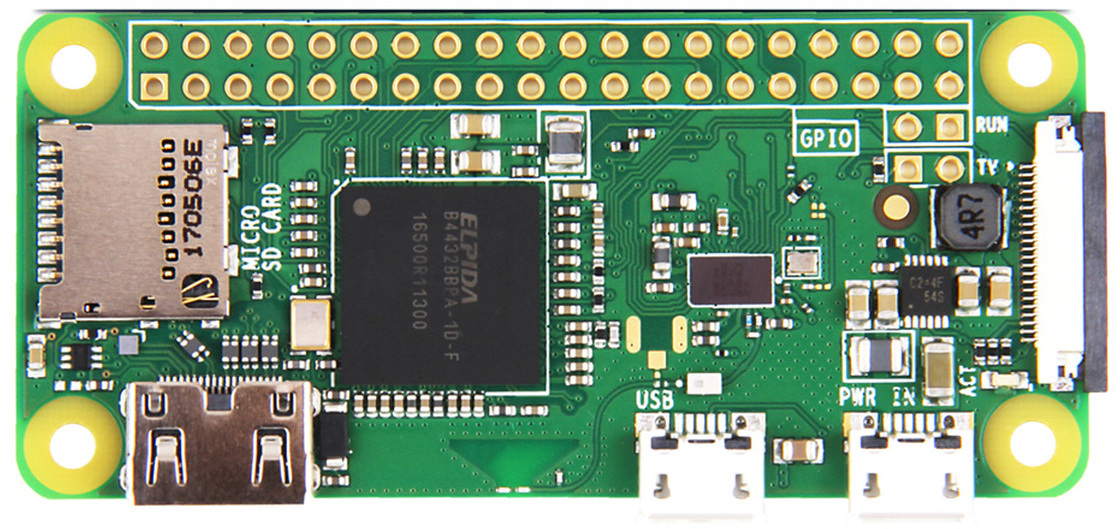
\includegraphics{Figures/Pi0W.jpg}\\[1 cm]	% University Logo
	\vfill
	\textsc{\LARGE EEE3096S/EEE3095S}\\[0.5 cm]				% Course Code
	\textsc{\large Embedded Systems II}\\[0.5 cm]				% Course Name
	\rule{\linewidth}{0.2 mm} \\[0.4 cm]
	{ \huge \bfseries Work Packages  2020}\\
	\rule{\linewidth}{0.2 mm} \\[1.5 cm]
    \vfill
	{\large \today}\\
\end{titlepage}

\begin{abstract}
Welcome to the practicals for EEE3096S. These instruction are applicable to all practicals so please take note! It is critical to do the pre-practical/tutorial work. 
Tutors will not help you with questions with answers that would have been known had you done the pre-practical work. 
The UCT EE Wiki (\href{wiki.ee.uct.ac.za}{wiki.ee.uct.ac.za}) is a very useful point to find any additional learning resources you might need. Use the search functionality on the top right of the page.

\subsection*{Practical Instructions}
\begin{itemize}
    \item \textbf{Naming}\\
    All files submitted to Vula need to be in the format. Marks will be deducted if not.
    \begin{lstlisting}[gobble=4]
    pracnum_studnum1_studnum2.fileformat
    \end{lstlisting}
    \item \textbf{Submission}
    \begin{itemize}
        \item Work packages consist of a tutorial and a practical. Be sure you submit to the correct submission on Vula!
        \item All text assignments must be submitted as pdf, and pdf only.
        \item Code within PDFs should not be as a screenshot, but as text. 
        \item Where appropriate, each pdf should contain a link to your GitHub repository.
    \end{itemize}
    \item \textbf{Groups}\\
    All practicals are to be completed in groups of 2. If a group of 2 can't be formed, permission will be needed to form a group of 3.
    \item \textbf{Bonus Marks}\\
    Occasionally, practicals will have ``bonus marks". If you do get bonus marks, the total marks for your prac cannot go over 100\%.
    \item \textbf{Mark Deductions}\\
    Occasionally, marks will be deducted from practicals. These will be conveyed to you in the practical, but many will be consistent across practicals, such as incorrectly names submissions or including code as a screenshot instead of formatted text.
    \item \textbf{Late Penalties}\\
    Late penalties will work as 10\% deduction per day, up to a maximum of 30\%. After this, you will receive 0\% and have the submission marked as incomplete.
    
\end{itemize}

\end{abstract}



\tableofcontents
\clearpage

% Debugging prac
\chapter{Work Package 1}
\section{Tutorial - Debugging using gdb}
By the end of this tutorial, we expect you to:
\begin{itemize}
    \item Be comfortable working in terminal/on the command line
    \item Understand real-time debugging
    \item Be familiar with at least 1 development and debugging tool-chain
\end{itemize}

\subsection{Requirements}
For this prac we'll be working with C/C++. In order to do so, you need to have a suitable compiler. Ubuntu and most linux Distros have this by default. On Windows however, you'll need MinGW. For a guide on how to install and configure that, visit \href{http://wiki.ee.uct.ac.za/MinGW}{this page} on the EE Wiki.


\subsection{Learning resources}
There's more information in these links than you will need for this practical, but they have been curated to make the information more relevant to you.

A quick overview of toolchains, makefiles and compilers:\footnote{The video covers details specific to 2019 Prac's 2 (this year's Prac 3!) but it serves as a reasonable overview to compilation. Don't worry if it's scary! We'll walk you through the process in this work package and future relevant work packages.}
\begin{itemize}
    \item \href{https://www.youtube.com/watch?v=XkITUjMg0s4}{https://www.youtube.com/watch?v=XkITUjMg0s4}
    \item \href{http://wiki.ee.uct.ac.za/Toolchains,_Compilers_And_Makefiles}{http://wiki.ee.uct.ac.za/Toolchains,\_Compilers\_And\_Makefiles}
\end{itemize} 


Information on gdb: 
\begin{itemize}
    \item \href{http://wiki.ee.uct.ac.za/GNU\_Debugger\_(GDB)}{http://wiki.ee.uct.ac.za/GNU\_Debugger\_(GDB)}
\end{itemize}

\subsection{Simple gdb walkthrough}
To learn about gsb, let's create a very simple\footnote{Incredibly simple.} calculator. 
\begin{enumerate}
    \item Create a file called ``main.c" on the command line:\\
        Ubuntu: \verb|$touch main.c|\\ 
        Windows: \verb|type nul > main.c|
    \item Open the file in your favourite editor.:\\
        Ubuntu: \verb|$nano main.c|\\
        Windows: \verb|notepad main.c|\\
        However it is recommended you use notepad++ which can be downloaded   \href{https://notepad-plus-plus.org/downloads/}{here}.\\
        To start notepad++ from the command line, use \verb|start notepad++ main.c|
        
    \item Inside it, place the following code:
        \begin{lstlisting}[gobble=8]
        # include <stdio.h>
        int main(){
	        int a, b, sum;

	        printf("Enter a value for a: ");
	        scanf("%d", &a);

	        printf("Enter a value for b: ");
	        scanf("%d", &a);

	        sum = a + b;

	        printf("The sum of a and b is %d \n.",sum);
        }
        \end{lstlisting}
    \item Compile it with the debugging flag:\\
        Ubuntu: \verb|$ gcc -g main.c|\\
        Windows: \verb|gcc -g main.c| \\ Note that this assumes you've correctly installed and configured MinGW
        
    \item Run it!\\
        Ubuntu: \verb|$ ./a.out|\\
        Windows: \verb|a.exe|\\
        If you try add two numbers - you'll see something really odd happen! Let's use \verb|gdb| to figure it out
   
    \item Open it in gdb:\\
        Ubuntu: \verb|$ gdb a.out|\\
        Windows: \verb|gdb.exe a.exe| 
    \item We need to add breakpoints. Let's add them at a points where we need to validate data:
    \begin{enumerate}
        \item Line 6 - once we have a value for a\\
        \verb|break 6|
        \item Line 9 - once we have a value for for b\\
        \verb|break 9|
        \item Line 12 - once we've added them together\\
        \verb|break 12|
    \end{enumerate}
    \item Run the application inside gdb!\\
    \verb|run|
    \begin{enumerate}
        \item You'll be prompted to enter in a value for a. Enter in something simple, such as 3
        \item Once you hit the enter key, gdb will step in. Let's print the value of a to ensure it is 3\\
        \verb|print a|
        \item If we're happy that it's the value we entered, we can continue execution by entering in \verb|c| and pressing enter.
        \item We're prompted for a value for b. Let's do another simple number, 5 \\(Please note Windows may not prompt you for the next number, but you can enter it anyway) %Austin
        \item gdb now steps in again. Let's validate that the value for b is indeed 5.\\
        \verb|print b|\\
        It's not! Let's double check the value of a with \verb|print a|\\
        The variable a was assigned the value of 5!
        \item We now know that when we enter out value for b, it's being assigned to a. We also know to look between lines 9 and 11 for our error. Close gdb by typing ``q" and pressing enter. You will be prompted to kill the debugging session, do so by typing ``y" and then pressing enter.
    \end{enumerate}
    \item Look for the error.\\
    Do you see it? Here's a hint: It was caused by a copy-paste that went unedited.\\
    That's right! Line 10 assigned the value entered for b to the variable a. As a result, a gets updated with the intended value for b, and, because b is never initialised or assigned, it holds a random value from whatever might be in memory.
    \item Fix up the error, and run the calculator again. It should now work as expected.
\end{enumerate}

\subsection{SPI questions}
The answers to the following need to be submitted to Vula in PDF format, with \verb|Tut1_<studnum1_studnum2.pdf| as the format.

\begin{enumerate}
    \item What do the following stand for? [3 marks]
    \begin{enumerate}
        \item MOSI % 1 mark
        \item MISO % 1 mark
        \item SCLK % 2 marks "Serial" and "clock"
    \end{enumerate}
    \item How might you connect multiple SPI devices on a single SPI bus? [3 marks]
    \item Draw a signal timing diagram showing the difference between the 2 different clock phase modes SPI can be configured to use. Only 2 bits of example data need to be shown in the timing diagrams [4 marks]\\
    Consider using \href{https://wavedrom.com/}{wavedrom.com}, though this is not a requirement.
\end{enumerate}
\section{Practical - ADC on the Pi}
Prac 5 is going to serve as an introduction to the mini-project, requiring you to configure some basic systems before integrating them all into the final device. Part of the deliverables for this prac is a short demo video which you could record on a smartphone and upload as part of the assignment, see Section \ref{prac4sub}.

In this prac you're going to sample temperature data from the ADC every 10 seconds. We're going to be using the \href{https://learn.adafruit.com/mcp3008-spi-adc/python-circuitpython}{Adafruit MCP3008 Library for Python}.

\subsection{Circuit}
You need to connect the following:
\begin{itemize}
    \item MCP3008 CLK to Pi SCLK
    \item MCP3008 DOUT to Pi MISO
    \item MCP3008 DIN to Pi MOSI
    \item MCP3008 CS/SHDN to Pi CE0
    \item MCP3008 VDD to Pi 3.3V
    \item MCP3008 VREF to Pi 3.3V
    \item MCP3008 AGND to Pi GND
    \item MCP3008 DGND to Pi GND
    \item Read the \href{http://ww1.microchip.com/downloads/en/DeviceDoc/20001942G.pdf}{data sheet for the MCP9700} and connect it correctly to channel 1 (pin 2) of the ADC.
    \item Add a button on a suitable GPIO pin
\end{itemize}

\begin{figure}[H]
\centering
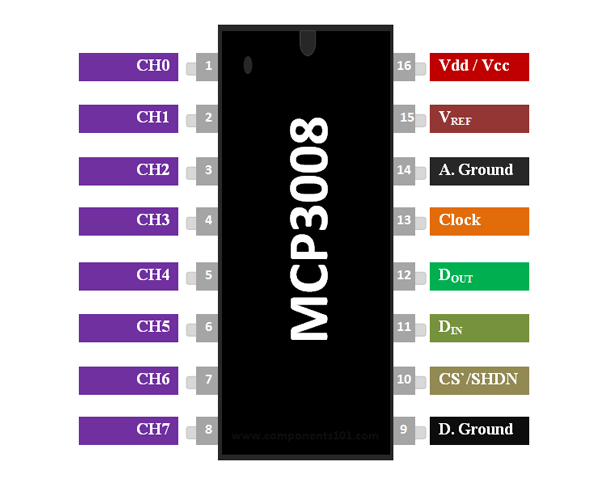
\includegraphics[width=0.6\columnwidth]{Figures/MCP3008Pinout}
\caption{The pinout of the MCP3008}
% \label{}
\end{figure}

\subsection{Walkthrough}
\begin{enumerate}
    \item Enable SPI using the raspi-config tool
    \item Install the MCP3008 Adafruit library
    \begin{lstlisting}[gobble=4]
    $ sudo apt-get update
    $ sudo apt install build-essential python3-dev python3-smbus python3-pip
    $ sudo pip3 install adafruit-circuitpython-mcp3xxx
    \end{lstlisting}
    \item Build the circuit described above.
    \item Create a new python file
    \item Place the following code in it:
    \begin{lstlisting} [gobble=4]
    import busio
    import digitalio
    import board
    import adafruit_mcp3xxx.mcp3008 as MCP
    from adafruit_mcp3xxx.analog_in import AnalogIn

    # create the spi bus
    spi = busio.SPI(clock=board.SCK, MISO=board.MISO, MOSI=board.MOSI)

    # create the cs (chip select)
    cs = digitalio.DigitalInOut(board.D5)

    # create the mcp object
    mcp = MCP.MCP3008(spi, cs)

    # create an analog input channel on pin 0
    chan = AnalogIn(mcp, MCP.P0)

    print('Raw ADC Value: ', chan.value)
    print('ADC Voltage: ' + str(chan.voltage) + 'V')
    \end{lstlisting}
    If you run this code you will see the reading from the LDR. Cover the sensor and run the code again. The reading should change.
    \item Adapt your code to read from both sensors and print to terminal every ten seconds. You \textbf{must} use a thread. You can read about simple threading in Python \href{http://wiki.ee.uct.ac.za/RaspberryPi:ProgrammingInPython}{here}. The output of your application should look as follows:
    \begin{lstlisting}[gobble=4]
    Runtime     Temp Reading    Temp	
    0s          <ADC value>	    <converted temp>  C
    10s         <ADC value>	    <converted temp>  C
    20s         <ADC value>	    <converted temp>  C
    30s         <ADC value>	    <converted temp>  C
    40s         <ADC value>	    <converted temp>  C
    50s         <ADC value>	    <converted temp>  C
    60s         <ADC value>	    <converted temp>  C
    \end{lstlisting}
    \item Runtime must be calculated, and not be implemented as a counter
    \item Add a button to toggle the rate of sampling between 10s, 5s and 1s
\end{enumerate}

\subsection{Requirements for submission}
\label{prac4sub}
There are two items you need to uploaded to Vula for submission of this practical assignment: 
\begin{enumerate}
    \item Your prac report provided as a single PDF file, named \verb|Prac5_<studnum1>_<studnum2>.pdf|
    \item A short demo video in which you present your design and implementation (see demo marking guide in Table \ref{tbl:Prac5DemoValidation} below).
\end{enumerate}


\textbf{Report Requirements}

The report should contain the following:
\begin{enumerate}
    \item The circuit diagram you used
    \item A paragraph on your validation and testing for the values you got from the ADC for both light and temperature
    \item Your Python code (screenshots of code will not be marked)
\end{enumerate}
Marks will be awarded for:
\begin{itemize}
    \item Neatness (circuit diagram and code)
    \item Correctness
    \item Using threads correctly
    \item Correct implementation of the temperature reading algorithm
\end{itemize}

\textbf{Demo Marking Guide}

Marks will be deducted for:
\begin{itemize}
    \item Not following instructions
    \item Plagiarism/Copying
\end{itemize}

You can prepare a short video, about 5 minutes will probably be sufficient. There is no minimum duration, but you need to respond to the aspects as listed in the marksheet below; but we do \textit{not} want videos beyond 10 minutes in length. The demo should respond to the following aspects (the marking allocations are shown on the right):

\label{sec:ProjAValidation}
\begin{table}[H]
\caption{The Mark sheet for the demo aspect of Prac5}
\label{tbl:Prac5DemoValidation}
\centering
\resizebox{\textwidth}{!}{%
\begin{tabular}{|l|l|l|r|c|}
\hline
% \multicolumn{3}{|l|}{{\ul \textbf{Project Validation Sheet}}}  & \multicolumn{2}{l|}{\begin{tabular}[c]{@{}l@{}}\textbf{Marked by:} \\ \\\end{tabular}} \\ \hline
% \multicolumn{7}{|l|}{\begin{tabular}[c]{@{}l@{}}\textbf{Student Numbers:} \\ \\ \\\end{tabular}} \\ \hline
\textbf{Category} & \textbf{Item} & \textbf{Description} & \multicolumn{1}{c|}{Max Mark} & \begin{tabular}[c]{@{}c@{}}Attempt\\ 1\end{tabular} \\ \hline 

\textbf{Intro} & \begin{tabular}[c]{@{}l@{}}Intro \\ and division of \\ workload \end{tabular} & \begin{tabular}[c]{@{}l@{}}Start off the demo by\\ indicating your prac team \\ members. \\ Indicate how you \\ divided up the work \end{tabular} & 6 &    \\ \hline

\textbf{Design} & Design and connections & \begin{tabular}[c]{@{}l@{}}Indicate the way\\ you hooked up the ADC \\ (using a circuit diagram or alternate \\ clear visualization) \\ and present the software design \\ e.g block diagram or flow chart \\ of your program \end{tabular} & 5 &  \\ \hline
 &  & \begin{tabular}[c]{@{}l@{}}Point to significant parts of \\ your code that \\ concerns the hardware and \\ any timing aspects \\ (use of comments,\\ and reminders in the \\ code, e.g. of things to draw \\ attention to in the demo are recommended)\end{tabular} & 5 &  \\ \hline
 
ADC Test & Testing Implementation & \begin{tabular}[c]{@{}l@{}}Run through the \\ operation of your \\ prototype  (e.g. increase light \\ decrease light, etc) \end{tabular} & 10 &  \\ \hline

%  & Potentiometer & \begin{tabular}[c]{@{}l@{}}Responds to changes input, \\ reading displayed is between\\ 0 and 3.3V\end{tabular} & 2 &  &  &  \\ \hline
Conclude & Conclude the presentation & \begin{tabular}[c]{@{}l@{}}Report on the extent the test was \\ successful provide some suggestions \\ for how you might improve \\ things or add features if time allowed \end{tabular} & 4 & \begin{tabular}[c]{@{}l@{}} \end{tabular}  \\ \hline
Mark &  &  & 30 & \begin{tabular}[c]{@{}l@{}} \\ \\\end{tabular} \\ \hline
\end{tabular}%
}
\end{table}



% ALU
\chapter{Work Package 2}
\section{Tutorial - Debugging using gdb}
By the end of this tutorial, we expect you to:
\begin{itemize}
    \item Be comfortable working in terminal/on the command line
    \item Understand real-time debugging
    \item Be familiar with at least 1 development and debugging tool-chain
\end{itemize}

\subsection{Requirements}
For this prac we'll be working with C/C++. In order to do so, you need to have a suitable compiler. Ubuntu and most linux Distros have this by default. On Windows however, you'll need MinGW. For a guide on how to install and configure that, visit \href{http://wiki.ee.uct.ac.za/MinGW}{this page} on the EE Wiki.


\subsection{Learning resources}
There's more information in these links than you will need for this practical, but they have been curated to make the information more relevant to you.

A quick overview of toolchains, makefiles and compilers:\footnote{The video covers details specific to 2019 Prac's 2 (this year's Prac 3!) but it serves as a reasonable overview to compilation. Don't worry if it's scary! We'll walk you through the process in this work package and future relevant work packages.}
\begin{itemize}
    \item \href{https://www.youtube.com/watch?v=XkITUjMg0s4}{https://www.youtube.com/watch?v=XkITUjMg0s4}
    \item \href{http://wiki.ee.uct.ac.za/Toolchains,_Compilers_And_Makefiles}{http://wiki.ee.uct.ac.za/Toolchains,\_Compilers\_And\_Makefiles}
\end{itemize} 


Information on gdb: 
\begin{itemize}
    \item \href{http://wiki.ee.uct.ac.za/GNU\_Debugger\_(GDB)}{http://wiki.ee.uct.ac.za/GNU\_Debugger\_(GDB)}
\end{itemize}

\subsection{Simple gdb walkthrough}
To learn about gsb, let's create a very simple\footnote{Incredibly simple.} calculator. 
\begin{enumerate}
    \item Create a file called ``main.c" on the command line:\\
        Ubuntu: \verb|$touch main.c|\\ 
        Windows: \verb|type nul > main.c|
    \item Open the file in your favourite editor.:\\
        Ubuntu: \verb|$nano main.c|\\
        Windows: \verb|notepad main.c|\\
        However it is recommended you use notepad++ which can be downloaded   \href{https://notepad-plus-plus.org/downloads/}{here}.\\
        To start notepad++ from the command line, use \verb|start notepad++ main.c|
        
    \item Inside it, place the following code:
        \begin{lstlisting}[gobble=8]
        # include <stdio.h>
        int main(){
	        int a, b, sum;

	        printf("Enter a value for a: ");
	        scanf("%d", &a);

	        printf("Enter a value for b: ");
	        scanf("%d", &a);

	        sum = a + b;

	        printf("The sum of a and b is %d \n.",sum);
        }
        \end{lstlisting}
    \item Compile it with the debugging flag:\\
        Ubuntu: \verb|$ gcc -g main.c|\\
        Windows: \verb|gcc -g main.c| \\ Note that this assumes you've correctly installed and configured MinGW
        
    \item Run it!\\
        Ubuntu: \verb|$ ./a.out|\\
        Windows: \verb|a.exe|\\
        If you try add two numbers - you'll see something really odd happen! Let's use \verb|gdb| to figure it out
   
    \item Open it in gdb:\\
        Ubuntu: \verb|$ gdb a.out|\\
        Windows: \verb|gdb.exe a.exe| 
    \item We need to add breakpoints. Let's add them at a points where we need to validate data:
    \begin{enumerate}
        \item Line 6 - once we have a value for a\\
        \verb|break 6|
        \item Line 9 - once we have a value for for b\\
        \verb|break 9|
        \item Line 12 - once we've added them together\\
        \verb|break 12|
    \end{enumerate}
    \item Run the application inside gdb!\\
    \verb|run|
    \begin{enumerate}
        \item You'll be prompted to enter in a value for a. Enter in something simple, such as 3
        \item Once you hit the enter key, gdb will step in. Let's print the value of a to ensure it is 3\\
        \verb|print a|
        \item If we're happy that it's the value we entered, we can continue execution by entering in \verb|c| and pressing enter.
        \item We're prompted for a value for b. Let's do another simple number, 5 \\(Please note Windows may not prompt you for the next number, but you can enter it anyway) %Austin
        \item gdb now steps in again. Let's validate that the value for b is indeed 5.\\
        \verb|print b|\\
        It's not! Let's double check the value of a with \verb|print a|\\
        The variable a was assigned the value of 5!
        \item We now know that when we enter out value for b, it's being assigned to a. We also know to look between lines 9 and 11 for our error. Close gdb by typing ``q" and pressing enter. You will be prompted to kill the debugging session, do so by typing ``y" and then pressing enter.
    \end{enumerate}
    \item Look for the error.\\
    Do you see it? Here's a hint: It was caused by a copy-paste that went unedited.\\
    That's right! Line 10 assigned the value entered for b to the variable a. As a result, a gets updated with the intended value for b, and, because b is never initialised or assigned, it holds a random value from whatever might be in memory.
    \item Fix up the error, and run the calculator again. It should now work as expected.
\end{enumerate}

\subsection{SPI questions}
The answers to the following need to be submitted to Vula in PDF format, with \verb|Tut1_<studnum1_studnum2.pdf| as the format.

\begin{enumerate}
    \item What do the following stand for? [3 marks]
    \begin{enumerate}
        \item MOSI % 1 mark
        \item MISO % 1 mark
        \item SCLK % 2 marks "Serial" and "clock"
    \end{enumerate}
    \item How might you connect multiple SPI devices on a single SPI bus? [3 marks]
    \item Draw a signal timing diagram showing the difference between the 2 different clock phase modes SPI can be configured to use. Only 2 bits of example data need to be shown in the timing diagrams [4 marks]\\
    Consider using \href{https://wavedrom.com/}{wavedrom.com}, though this is not a requirement.
\end{enumerate}
\section{Practical - ADC on the Pi}
Prac 5 is going to serve as an introduction to the mini-project, requiring you to configure some basic systems before integrating them all into the final device. Part of the deliverables for this prac is a short demo video which you could record on a smartphone and upload as part of the assignment, see Section \ref{prac4sub}.

In this prac you're going to sample temperature data from the ADC every 10 seconds. We're going to be using the \href{https://learn.adafruit.com/mcp3008-spi-adc/python-circuitpython}{Adafruit MCP3008 Library for Python}.

\subsection{Circuit}
You need to connect the following:
\begin{itemize}
    \item MCP3008 CLK to Pi SCLK
    \item MCP3008 DOUT to Pi MISO
    \item MCP3008 DIN to Pi MOSI
    \item MCP3008 CS/SHDN to Pi CE0
    \item MCP3008 VDD to Pi 3.3V
    \item MCP3008 VREF to Pi 3.3V
    \item MCP3008 AGND to Pi GND
    \item MCP3008 DGND to Pi GND
    \item Read the \href{http://ww1.microchip.com/downloads/en/DeviceDoc/20001942G.pdf}{data sheet for the MCP9700} and connect it correctly to channel 1 (pin 2) of the ADC.
    \item Add a button on a suitable GPIO pin
\end{itemize}

\begin{figure}[H]
\centering
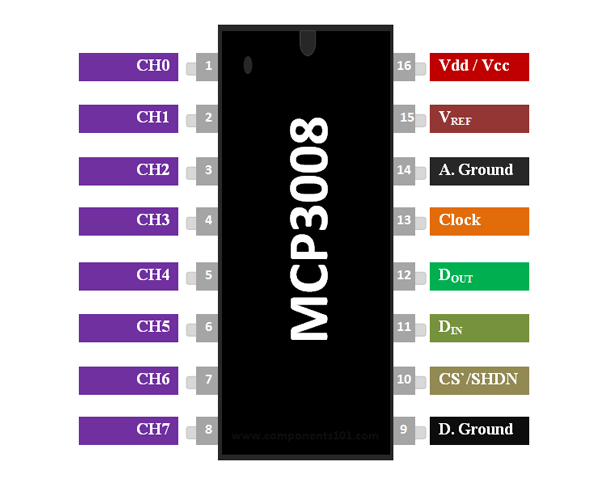
\includegraphics[width=0.6\columnwidth]{Figures/MCP3008Pinout}
\caption{The pinout of the MCP3008}
% \label{}
\end{figure}

\subsection{Walkthrough}
\begin{enumerate}
    \item Enable SPI using the raspi-config tool
    \item Install the MCP3008 Adafruit library
    \begin{lstlisting}[gobble=4]
    $ sudo apt-get update
    $ sudo apt install build-essential python3-dev python3-smbus python3-pip
    $ sudo pip3 install adafruit-circuitpython-mcp3xxx
    \end{lstlisting}
    \item Build the circuit described above.
    \item Create a new python file
    \item Place the following code in it:
    \begin{lstlisting} [gobble=4]
    import busio
    import digitalio
    import board
    import adafruit_mcp3xxx.mcp3008 as MCP
    from adafruit_mcp3xxx.analog_in import AnalogIn

    # create the spi bus
    spi = busio.SPI(clock=board.SCK, MISO=board.MISO, MOSI=board.MOSI)

    # create the cs (chip select)
    cs = digitalio.DigitalInOut(board.D5)

    # create the mcp object
    mcp = MCP.MCP3008(spi, cs)

    # create an analog input channel on pin 0
    chan = AnalogIn(mcp, MCP.P0)

    print('Raw ADC Value: ', chan.value)
    print('ADC Voltage: ' + str(chan.voltage) + 'V')
    \end{lstlisting}
    If you run this code you will see the reading from the LDR. Cover the sensor and run the code again. The reading should change.
    \item Adapt your code to read from both sensors and print to terminal every ten seconds. You \textbf{must} use a thread. You can read about simple threading in Python \href{http://wiki.ee.uct.ac.za/RaspberryPi:ProgrammingInPython}{here}. The output of your application should look as follows:
    \begin{lstlisting}[gobble=4]
    Runtime     Temp Reading    Temp	
    0s          <ADC value>	    <converted temp>  C
    10s         <ADC value>	    <converted temp>  C
    20s         <ADC value>	    <converted temp>  C
    30s         <ADC value>	    <converted temp>  C
    40s         <ADC value>	    <converted temp>  C
    50s         <ADC value>	    <converted temp>  C
    60s         <ADC value>	    <converted temp>  C
    \end{lstlisting}
    \item Runtime must be calculated, and not be implemented as a counter
    \item Add a button to toggle the rate of sampling between 10s, 5s and 1s
\end{enumerate}

\subsection{Requirements for submission}
\label{prac4sub}
There are two items you need to uploaded to Vula for submission of this practical assignment: 
\begin{enumerate}
    \item Your prac report provided as a single PDF file, named \verb|Prac5_<studnum1>_<studnum2>.pdf|
    \item A short demo video in which you present your design and implementation (see demo marking guide in Table \ref{tbl:Prac5DemoValidation} below).
\end{enumerate}


\textbf{Report Requirements}

The report should contain the following:
\begin{enumerate}
    \item The circuit diagram you used
    \item A paragraph on your validation and testing for the values you got from the ADC for both light and temperature
    \item Your Python code (screenshots of code will not be marked)
\end{enumerate}
Marks will be awarded for:
\begin{itemize}
    \item Neatness (circuit diagram and code)
    \item Correctness
    \item Using threads correctly
    \item Correct implementation of the temperature reading algorithm
\end{itemize}

\textbf{Demo Marking Guide}

Marks will be deducted for:
\begin{itemize}
    \item Not following instructions
    \item Plagiarism/Copying
\end{itemize}

You can prepare a short video, about 5 minutes will probably be sufficient. There is no minimum duration, but you need to respond to the aspects as listed in the marksheet below; but we do \textit{not} want videos beyond 10 minutes in length. The demo should respond to the following aspects (the marking allocations are shown on the right):

\label{sec:ProjAValidation}
\begin{table}[H]
\caption{The Mark sheet for the demo aspect of Prac5}
\label{tbl:Prac5DemoValidation}
\centering
\resizebox{\textwidth}{!}{%
\begin{tabular}{|l|l|l|r|c|}
\hline
% \multicolumn{3}{|l|}{{\ul \textbf{Project Validation Sheet}}}  & \multicolumn{2}{l|}{\begin{tabular}[c]{@{}l@{}}\textbf{Marked by:} \\ \\\end{tabular}} \\ \hline
% \multicolumn{7}{|l|}{\begin{tabular}[c]{@{}l@{}}\textbf{Student Numbers:} \\ \\ \\\end{tabular}} \\ \hline
\textbf{Category} & \textbf{Item} & \textbf{Description} & \multicolumn{1}{c|}{Max Mark} & \begin{tabular}[c]{@{}c@{}}Attempt\\ 1\end{tabular} \\ \hline 

\textbf{Intro} & \begin{tabular}[c]{@{}l@{}}Intro \\ and division of \\ workload \end{tabular} & \begin{tabular}[c]{@{}l@{}}Start off the demo by\\ indicating your prac team \\ members. \\ Indicate how you \\ divided up the work \end{tabular} & 6 &    \\ \hline

\textbf{Design} & Design and connections & \begin{tabular}[c]{@{}l@{}}Indicate the way\\ you hooked up the ADC \\ (using a circuit diagram or alternate \\ clear visualization) \\ and present the software design \\ e.g block diagram or flow chart \\ of your program \end{tabular} & 5 &  \\ \hline
 &  & \begin{tabular}[c]{@{}l@{}}Point to significant parts of \\ your code that \\ concerns the hardware and \\ any timing aspects \\ (use of comments,\\ and reminders in the \\ code, e.g. of things to draw \\ attention to in the demo are recommended)\end{tabular} & 5 &  \\ \hline
 
ADC Test & Testing Implementation & \begin{tabular}[c]{@{}l@{}}Run through the \\ operation of your \\ prototype  (e.g. increase light \\ decrease light, etc) \end{tabular} & 10 &  \\ \hline

%  & Potentiometer & \begin{tabular}[c]{@{}l@{}}Responds to changes input, \\ reading displayed is between\\ 0 and 3.3V\end{tabular} & 2 &  &  &  \\ \hline
Conclude & Conclude the presentation & \begin{tabular}[c]{@{}l@{}}Report on the extent the test was \\ successful provide some suggestions \\ for how you might improve \\ things or add features if time allowed \end{tabular} & 4 & \begin{tabular}[c]{@{}l@{}} \end{tabular}  \\ \hline
Mark &  &  & 30 & \begin{tabular}[c]{@{}l@{}} \\ \\\end{tabular} \\ \hline
\end{tabular}%
}
\end{table}



% First RPi Prac - Benchmarking & Intro
 \chapter{Work Package 3}
 \section{Tutorial - Debugging using gdb}
By the end of this tutorial, we expect you to:
\begin{itemize}
    \item Be comfortable working in terminal/on the command line
    \item Understand real-time debugging
    \item Be familiar with at least 1 development and debugging tool-chain
\end{itemize}

\subsection{Requirements}
For this prac we'll be working with C/C++. In order to do so, you need to have a suitable compiler. Ubuntu and most linux Distros have this by default. On Windows however, you'll need MinGW. For a guide on how to install and configure that, visit \href{http://wiki.ee.uct.ac.za/MinGW}{this page} on the EE Wiki.


\subsection{Learning resources}
There's more information in these links than you will need for this practical, but they have been curated to make the information more relevant to you.

A quick overview of toolchains, makefiles and compilers:\footnote{The video covers details specific to 2019 Prac's 2 (this year's Prac 3!) but it serves as a reasonable overview to compilation. Don't worry if it's scary! We'll walk you through the process in this work package and future relevant work packages.}
\begin{itemize}
    \item \href{https://www.youtube.com/watch?v=XkITUjMg0s4}{https://www.youtube.com/watch?v=XkITUjMg0s4}
    \item \href{http://wiki.ee.uct.ac.za/Toolchains,_Compilers_And_Makefiles}{http://wiki.ee.uct.ac.za/Toolchains,\_Compilers\_And\_Makefiles}
\end{itemize} 


Information on gdb: 
\begin{itemize}
    \item \href{http://wiki.ee.uct.ac.za/GNU\_Debugger\_(GDB)}{http://wiki.ee.uct.ac.za/GNU\_Debugger\_(GDB)}
\end{itemize}

\subsection{Simple gdb walkthrough}
To learn about gsb, let's create a very simple\footnote{Incredibly simple.} calculator. 
\begin{enumerate}
    \item Create a file called ``main.c" on the command line:\\
        Ubuntu: \verb|$touch main.c|\\ 
        Windows: \verb|type nul > main.c|
    \item Open the file in your favourite editor.:\\
        Ubuntu: \verb|$nano main.c|\\
        Windows: \verb|notepad main.c|\\
        However it is recommended you use notepad++ which can be downloaded   \href{https://notepad-plus-plus.org/downloads/}{here}.\\
        To start notepad++ from the command line, use \verb|start notepad++ main.c|
        
    \item Inside it, place the following code:
        \begin{lstlisting}[gobble=8]
        # include <stdio.h>
        int main(){
	        int a, b, sum;

	        printf("Enter a value for a: ");
	        scanf("%d", &a);

	        printf("Enter a value for b: ");
	        scanf("%d", &a);

	        sum = a + b;

	        printf("The sum of a and b is %d \n.",sum);
        }
        \end{lstlisting}
    \item Compile it with the debugging flag:\\
        Ubuntu: \verb|$ gcc -g main.c|\\
        Windows: \verb|gcc -g main.c| \\ Note that this assumes you've correctly installed and configured MinGW
        
    \item Run it!\\
        Ubuntu: \verb|$ ./a.out|\\
        Windows: \verb|a.exe|\\
        If you try add two numbers - you'll see something really odd happen! Let's use \verb|gdb| to figure it out
   
    \item Open it in gdb:\\
        Ubuntu: \verb|$ gdb a.out|\\
        Windows: \verb|gdb.exe a.exe| 
    \item We need to add breakpoints. Let's add them at a points where we need to validate data:
    \begin{enumerate}
        \item Line 6 - once we have a value for a\\
        \verb|break 6|
        \item Line 9 - once we have a value for for b\\
        \verb|break 9|
        \item Line 12 - once we've added them together\\
        \verb|break 12|
    \end{enumerate}
    \item Run the application inside gdb!\\
    \verb|run|
    \begin{enumerate}
        \item You'll be prompted to enter in a value for a. Enter in something simple, such as 3
        \item Once you hit the enter key, gdb will step in. Let's print the value of a to ensure it is 3\\
        \verb|print a|
        \item If we're happy that it's the value we entered, we can continue execution by entering in \verb|c| and pressing enter.
        \item We're prompted for a value for b. Let's do another simple number, 5 \\(Please note Windows may not prompt you for the next number, but you can enter it anyway) %Austin
        \item gdb now steps in again. Let's validate that the value for b is indeed 5.\\
        \verb|print b|\\
        It's not! Let's double check the value of a with \verb|print a|\\
        The variable a was assigned the value of 5!
        \item We now know that when we enter out value for b, it's being assigned to a. We also know to look between lines 9 and 11 for our error. Close gdb by typing ``q" and pressing enter. You will be prompted to kill the debugging session, do so by typing ``y" and then pressing enter.
    \end{enumerate}
    \item Look for the error.\\
    Do you see it? Here's a hint: It was caused by a copy-paste that went unedited.\\
    That's right! Line 10 assigned the value entered for b to the variable a. As a result, a gets updated with the intended value for b, and, because b is never initialised or assigned, it holds a random value from whatever might be in memory.
    \item Fix up the error, and run the calculator again. It should now work as expected.
\end{enumerate}

\subsection{SPI questions}
The answers to the following need to be submitted to Vula in PDF format, with \verb|Tut1_<studnum1_studnum2.pdf| as the format.

\begin{enumerate}
    \item What do the following stand for? [3 marks]
    \begin{enumerate}
        \item MOSI % 1 mark
        \item MISO % 1 mark
        \item SCLK % 2 marks "Serial" and "clock"
    \end{enumerate}
    \item How might you connect multiple SPI devices on a single SPI bus? [3 marks]
    \item Draw a signal timing diagram showing the difference between the 2 different clock phase modes SPI can be configured to use. Only 2 bits of example data need to be shown in the timing diagrams [4 marks]\\
    Consider using \href{https://wavedrom.com/}{wavedrom.com}, though this is not a requirement.
\end{enumerate} % Introduces students to BASH, git, etc
 \section{Practical - ADC on the Pi}
Prac 5 is going to serve as an introduction to the mini-project, requiring you to configure some basic systems before integrating them all into the final device. Part of the deliverables for this prac is a short demo video which you could record on a smartphone and upload as part of the assignment, see Section \ref{prac4sub}.

In this prac you're going to sample temperature data from the ADC every 10 seconds. We're going to be using the \href{https://learn.adafruit.com/mcp3008-spi-adc/python-circuitpython}{Adafruit MCP3008 Library for Python}.

\subsection{Circuit}
You need to connect the following:
\begin{itemize}
    \item MCP3008 CLK to Pi SCLK
    \item MCP3008 DOUT to Pi MISO
    \item MCP3008 DIN to Pi MOSI
    \item MCP3008 CS/SHDN to Pi CE0
    \item MCP3008 VDD to Pi 3.3V
    \item MCP3008 VREF to Pi 3.3V
    \item MCP3008 AGND to Pi GND
    \item MCP3008 DGND to Pi GND
    \item Read the \href{http://ww1.microchip.com/downloads/en/DeviceDoc/20001942G.pdf}{data sheet for the MCP9700} and connect it correctly to channel 1 (pin 2) of the ADC.
    \item Add a button on a suitable GPIO pin
\end{itemize}

\begin{figure}[H]
\centering
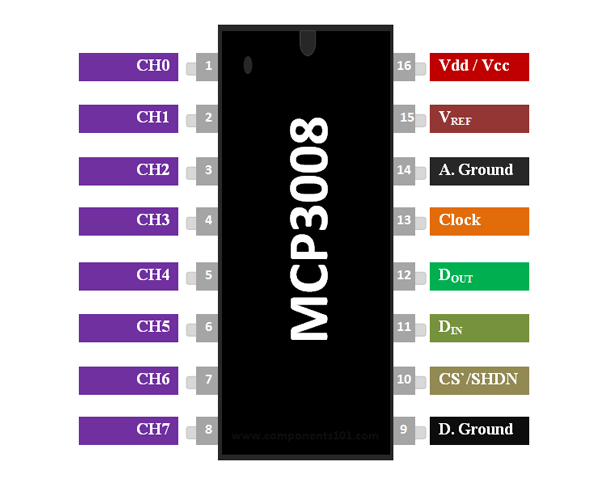
\includegraphics[width=0.6\columnwidth]{Figures/MCP3008Pinout}
\caption{The pinout of the MCP3008}
% \label{}
\end{figure}

\subsection{Walkthrough}
\begin{enumerate}
    \item Enable SPI using the raspi-config tool
    \item Install the MCP3008 Adafruit library
    \begin{lstlisting}[gobble=4]
    $ sudo apt-get update
    $ sudo apt install build-essential python3-dev python3-smbus python3-pip
    $ sudo pip3 install adafruit-circuitpython-mcp3xxx
    \end{lstlisting}
    \item Build the circuit described above.
    \item Create a new python file
    \item Place the following code in it:
    \begin{lstlisting} [gobble=4]
    import busio
    import digitalio
    import board
    import adafruit_mcp3xxx.mcp3008 as MCP
    from adafruit_mcp3xxx.analog_in import AnalogIn

    # create the spi bus
    spi = busio.SPI(clock=board.SCK, MISO=board.MISO, MOSI=board.MOSI)

    # create the cs (chip select)
    cs = digitalio.DigitalInOut(board.D5)

    # create the mcp object
    mcp = MCP.MCP3008(spi, cs)

    # create an analog input channel on pin 0
    chan = AnalogIn(mcp, MCP.P0)

    print('Raw ADC Value: ', chan.value)
    print('ADC Voltage: ' + str(chan.voltage) + 'V')
    \end{lstlisting}
    If you run this code you will see the reading from the LDR. Cover the sensor and run the code again. The reading should change.
    \item Adapt your code to read from both sensors and print to terminal every ten seconds. You \textbf{must} use a thread. You can read about simple threading in Python \href{http://wiki.ee.uct.ac.za/RaspberryPi:ProgrammingInPython}{here}. The output of your application should look as follows:
    \begin{lstlisting}[gobble=4]
    Runtime     Temp Reading    Temp	
    0s          <ADC value>	    <converted temp>  C
    10s         <ADC value>	    <converted temp>  C
    20s         <ADC value>	    <converted temp>  C
    30s         <ADC value>	    <converted temp>  C
    40s         <ADC value>	    <converted temp>  C
    50s         <ADC value>	    <converted temp>  C
    60s         <ADC value>	    <converted temp>  C
    \end{lstlisting}
    \item Runtime must be calculated, and not be implemented as a counter
    \item Add a button to toggle the rate of sampling between 10s, 5s and 1s
\end{enumerate}

\subsection{Requirements for submission}
\label{prac4sub}
There are two items you need to uploaded to Vula for submission of this practical assignment: 
\begin{enumerate}
    \item Your prac report provided as a single PDF file, named \verb|Prac5_<studnum1>_<studnum2>.pdf|
    \item A short demo video in which you present your design and implementation (see demo marking guide in Table \ref{tbl:Prac5DemoValidation} below).
\end{enumerate}


\textbf{Report Requirements}

The report should contain the following:
\begin{enumerate}
    \item The circuit diagram you used
    \item A paragraph on your validation and testing for the values you got from the ADC for both light and temperature
    \item Your Python code (screenshots of code will not be marked)
\end{enumerate}
Marks will be awarded for:
\begin{itemize}
    \item Neatness (circuit diagram and code)
    \item Correctness
    \item Using threads correctly
    \item Correct implementation of the temperature reading algorithm
\end{itemize}

\textbf{Demo Marking Guide}

Marks will be deducted for:
\begin{itemize}
    \item Not following instructions
    \item Plagiarism/Copying
\end{itemize}

You can prepare a short video, about 5 minutes will probably be sufficient. There is no minimum duration, but you need to respond to the aspects as listed in the marksheet below; but we do \textit{not} want videos beyond 10 minutes in length. The demo should respond to the following aspects (the marking allocations are shown on the right):

\label{sec:ProjAValidation}
\begin{table}[H]
\caption{The Mark sheet for the demo aspect of Prac5}
\label{tbl:Prac5DemoValidation}
\centering
\resizebox{\textwidth}{!}{%
\begin{tabular}{|l|l|l|r|c|}
\hline
% \multicolumn{3}{|l|}{{\ul \textbf{Project Validation Sheet}}}  & \multicolumn{2}{l|}{\begin{tabular}[c]{@{}l@{}}\textbf{Marked by:} \\ \\\end{tabular}} \\ \hline
% \multicolumn{7}{|l|}{\begin{tabular}[c]{@{}l@{}}\textbf{Student Numbers:} \\ \\ \\\end{tabular}} \\ \hline
\textbf{Category} & \textbf{Item} & \textbf{Description} & \multicolumn{1}{c|}{Max Mark} & \begin{tabular}[c]{@{}c@{}}Attempt\\ 1\end{tabular} \\ \hline 

\textbf{Intro} & \begin{tabular}[c]{@{}l@{}}Intro \\ and division of \\ workload \end{tabular} & \begin{tabular}[c]{@{}l@{}}Start off the demo by\\ indicating your prac team \\ members. \\ Indicate how you \\ divided up the work \end{tabular} & 6 &    \\ \hline

\textbf{Design} & Design and connections & \begin{tabular}[c]{@{}l@{}}Indicate the way\\ you hooked up the ADC \\ (using a circuit diagram or alternate \\ clear visualization) \\ and present the software design \\ e.g block diagram or flow chart \\ of your program \end{tabular} & 5 &  \\ \hline
 &  & \begin{tabular}[c]{@{}l@{}}Point to significant parts of \\ your code that \\ concerns the hardware and \\ any timing aspects \\ (use of comments,\\ and reminders in the \\ code, e.g. of things to draw \\ attention to in the demo are recommended)\end{tabular} & 5 &  \\ \hline
 
ADC Test & Testing Implementation & \begin{tabular}[c]{@{}l@{}}Run through the \\ operation of your \\ prototype  (e.g. increase light \\ decrease light, etc) \end{tabular} & 10 &  \\ \hline

%  & Potentiometer & \begin{tabular}[c]{@{}l@{}}Responds to changes input, \\ reading displayed is between\\ 0 and 3.3V\end{tabular} & 2 &  &  &  \\ \hline
Conclude & Conclude the presentation & \begin{tabular}[c]{@{}l@{}}Report on the extent the test was \\ successful provide some suggestions \\ for how you might improve \\ things or add features if time allowed \end{tabular} & 4 & \begin{tabular}[c]{@{}l@{}} \end{tabular}  \\ \hline
Mark &  &  & 30 & \begin{tabular}[c]{@{}l@{}} \\ \\\end{tabular} \\ \hline
\end{tabular}%
}
\end{table}

 % Heterodyning, C/C++ vs Python


% I2C, PWM and the RTC
\chapter{Work Package 4}
This work package details information on some good practice when working with embedded systems, such as debouncing, call backs, pull up and pull down logic, as well as more interesting concepts such as pulse width modulation, I2C and EEPROM. For the tutorial you will be required to do some research and answer some simple questions. For the practical you will make a simple number-guessing game.
\section{Tutorial - Debugging using gdb}
By the end of this tutorial, we expect you to:
\begin{itemize}
    \item Be comfortable working in terminal/on the command line
    \item Understand real-time debugging
    \item Be familiar with at least 1 development and debugging tool-chain
\end{itemize}

\subsection{Requirements}
For this prac we'll be working with C/C++. In order to do so, you need to have a suitable compiler. Ubuntu and most linux Distros have this by default. On Windows however, you'll need MinGW. For a guide on how to install and configure that, visit \href{http://wiki.ee.uct.ac.za/MinGW}{this page} on the EE Wiki.


\subsection{Learning resources}
There's more information in these links than you will need for this practical, but they have been curated to make the information more relevant to you.

A quick overview of toolchains, makefiles and compilers:\footnote{The video covers details specific to 2019 Prac's 2 (this year's Prac 3!) but it serves as a reasonable overview to compilation. Don't worry if it's scary! We'll walk you through the process in this work package and future relevant work packages.}
\begin{itemize}
    \item \href{https://www.youtube.com/watch?v=XkITUjMg0s4}{https://www.youtube.com/watch?v=XkITUjMg0s4}
    \item \href{http://wiki.ee.uct.ac.za/Toolchains,_Compilers_And_Makefiles}{http://wiki.ee.uct.ac.za/Toolchains,\_Compilers\_And\_Makefiles}
\end{itemize} 


Information on gdb: 
\begin{itemize}
    \item \href{http://wiki.ee.uct.ac.za/GNU\_Debugger\_(GDB)}{http://wiki.ee.uct.ac.za/GNU\_Debugger\_(GDB)}
\end{itemize}

\subsection{Simple gdb walkthrough}
To learn about gsb, let's create a very simple\footnote{Incredibly simple.} calculator. 
\begin{enumerate}
    \item Create a file called ``main.c" on the command line:\\
        Ubuntu: \verb|$touch main.c|\\ 
        Windows: \verb|type nul > main.c|
    \item Open the file in your favourite editor.:\\
        Ubuntu: \verb|$nano main.c|\\
        Windows: \verb|notepad main.c|\\
        However it is recommended you use notepad++ which can be downloaded   \href{https://notepad-plus-plus.org/downloads/}{here}.\\
        To start notepad++ from the command line, use \verb|start notepad++ main.c|
        
    \item Inside it, place the following code:
        \begin{lstlisting}[gobble=8]
        # include <stdio.h>
        int main(){
	        int a, b, sum;

	        printf("Enter a value for a: ");
	        scanf("%d", &a);

	        printf("Enter a value for b: ");
	        scanf("%d", &a);

	        sum = a + b;

	        printf("The sum of a and b is %d \n.",sum);
        }
        \end{lstlisting}
    \item Compile it with the debugging flag:\\
        Ubuntu: \verb|$ gcc -g main.c|\\
        Windows: \verb|gcc -g main.c| \\ Note that this assumes you've correctly installed and configured MinGW
        
    \item Run it!\\
        Ubuntu: \verb|$ ./a.out|\\
        Windows: \verb|a.exe|\\
        If you try add two numbers - you'll see something really odd happen! Let's use \verb|gdb| to figure it out
   
    \item Open it in gdb:\\
        Ubuntu: \verb|$ gdb a.out|\\
        Windows: \verb|gdb.exe a.exe| 
    \item We need to add breakpoints. Let's add them at a points where we need to validate data:
    \begin{enumerate}
        \item Line 6 - once we have a value for a\\
        \verb|break 6|
        \item Line 9 - once we have a value for for b\\
        \verb|break 9|
        \item Line 12 - once we've added them together\\
        \verb|break 12|
    \end{enumerate}
    \item Run the application inside gdb!\\
    \verb|run|
    \begin{enumerate}
        \item You'll be prompted to enter in a value for a. Enter in something simple, such as 3
        \item Once you hit the enter key, gdb will step in. Let's print the value of a to ensure it is 3\\
        \verb|print a|
        \item If we're happy that it's the value we entered, we can continue execution by entering in \verb|c| and pressing enter.
        \item We're prompted for a value for b. Let's do another simple number, 5 \\(Please note Windows may not prompt you for the next number, but you can enter it anyway) %Austin
        \item gdb now steps in again. Let's validate that the value for b is indeed 5.\\
        \verb|print b|\\
        It's not! Let's double check the value of a with \verb|print a|\\
        The variable a was assigned the value of 5!
        \item We now know that when we enter out value for b, it's being assigned to a. We also know to look between lines 9 and 11 for our error. Close gdb by typing ``q" and pressing enter. You will be prompted to kill the debugging session, do so by typing ``y" and then pressing enter.
    \end{enumerate}
    \item Look for the error.\\
    Do you see it? Here's a hint: It was caused by a copy-paste that went unedited.\\
    That's right! Line 10 assigned the value entered for b to the variable a. As a result, a gets updated with the intended value for b, and, because b is never initialised or assigned, it holds a random value from whatever might be in memory.
    \item Fix up the error, and run the calculator again. It should now work as expected.
\end{enumerate}

\subsection{SPI questions}
The answers to the following need to be submitted to Vula in PDF format, with \verb|Tut1_<studnum1_studnum2.pdf| as the format.

\begin{enumerate}
    \item What do the following stand for? [3 marks]
    \begin{enumerate}
        \item MOSI % 1 mark
        \item MISO % 1 mark
        \item SCLK % 2 marks "Serial" and "clock"
    \end{enumerate}
    \item How might you connect multiple SPI devices on a single SPI bus? [3 marks]
    \item Draw a signal timing diagram showing the difference between the 2 different clock phase modes SPI can be configured to use. Only 2 bits of example data need to be shown in the timing diagrams [4 marks]\\
    Consider using \href{https://wavedrom.com/}{wavedrom.com}, though this is not a requirement.
\end{enumerate}
\section{Practical - ADC on the Pi}
Prac 5 is going to serve as an introduction to the mini-project, requiring you to configure some basic systems before integrating them all into the final device. Part of the deliverables for this prac is a short demo video which you could record on a smartphone and upload as part of the assignment, see Section \ref{prac4sub}.

In this prac you're going to sample temperature data from the ADC every 10 seconds. We're going to be using the \href{https://learn.adafruit.com/mcp3008-spi-adc/python-circuitpython}{Adafruit MCP3008 Library for Python}.

\subsection{Circuit}
You need to connect the following:
\begin{itemize}
    \item MCP3008 CLK to Pi SCLK
    \item MCP3008 DOUT to Pi MISO
    \item MCP3008 DIN to Pi MOSI
    \item MCP3008 CS/SHDN to Pi CE0
    \item MCP3008 VDD to Pi 3.3V
    \item MCP3008 VREF to Pi 3.3V
    \item MCP3008 AGND to Pi GND
    \item MCP3008 DGND to Pi GND
    \item Read the \href{http://ww1.microchip.com/downloads/en/DeviceDoc/20001942G.pdf}{data sheet for the MCP9700} and connect it correctly to channel 1 (pin 2) of the ADC.
    \item Add a button on a suitable GPIO pin
\end{itemize}

\begin{figure}[H]
\centering
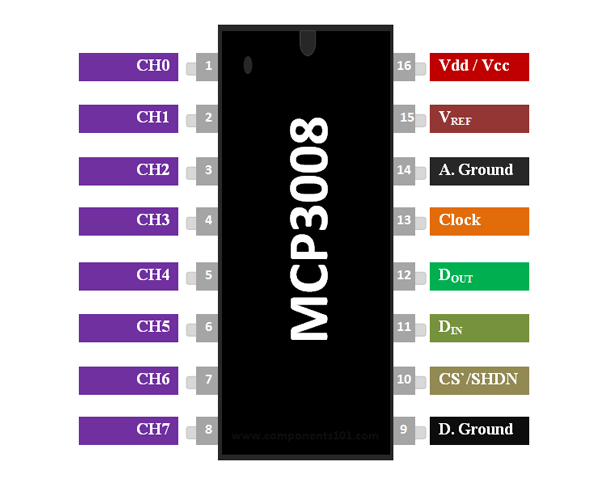
\includegraphics[width=0.6\columnwidth]{Figures/MCP3008Pinout}
\caption{The pinout of the MCP3008}
% \label{}
\end{figure}

\subsection{Walkthrough}
\begin{enumerate}
    \item Enable SPI using the raspi-config tool
    \item Install the MCP3008 Adafruit library
    \begin{lstlisting}[gobble=4]
    $ sudo apt-get update
    $ sudo apt install build-essential python3-dev python3-smbus python3-pip
    $ sudo pip3 install adafruit-circuitpython-mcp3xxx
    \end{lstlisting}
    \item Build the circuit described above.
    \item Create a new python file
    \item Place the following code in it:
    \begin{lstlisting} [gobble=4]
    import busio
    import digitalio
    import board
    import adafruit_mcp3xxx.mcp3008 as MCP
    from adafruit_mcp3xxx.analog_in import AnalogIn

    # create the spi bus
    spi = busio.SPI(clock=board.SCK, MISO=board.MISO, MOSI=board.MOSI)

    # create the cs (chip select)
    cs = digitalio.DigitalInOut(board.D5)

    # create the mcp object
    mcp = MCP.MCP3008(spi, cs)

    # create an analog input channel on pin 0
    chan = AnalogIn(mcp, MCP.P0)

    print('Raw ADC Value: ', chan.value)
    print('ADC Voltage: ' + str(chan.voltage) + 'V')
    \end{lstlisting}
    If you run this code you will see the reading from the LDR. Cover the sensor and run the code again. The reading should change.
    \item Adapt your code to read from both sensors and print to terminal every ten seconds. You \textbf{must} use a thread. You can read about simple threading in Python \href{http://wiki.ee.uct.ac.za/RaspberryPi:ProgrammingInPython}{here}. The output of your application should look as follows:
    \begin{lstlisting}[gobble=4]
    Runtime     Temp Reading    Temp	
    0s          <ADC value>	    <converted temp>  C
    10s         <ADC value>	    <converted temp>  C
    20s         <ADC value>	    <converted temp>  C
    30s         <ADC value>	    <converted temp>  C
    40s         <ADC value>	    <converted temp>  C
    50s         <ADC value>	    <converted temp>  C
    60s         <ADC value>	    <converted temp>  C
    \end{lstlisting}
    \item Runtime must be calculated, and not be implemented as a counter
    \item Add a button to toggle the rate of sampling between 10s, 5s and 1s
\end{enumerate}

\subsection{Requirements for submission}
\label{prac4sub}
There are two items you need to uploaded to Vula for submission of this practical assignment: 
\begin{enumerate}
    \item Your prac report provided as a single PDF file, named \verb|Prac5_<studnum1>_<studnum2>.pdf|
    \item A short demo video in which you present your design and implementation (see demo marking guide in Table \ref{tbl:Prac5DemoValidation} below).
\end{enumerate}


\textbf{Report Requirements}

The report should contain the following:
\begin{enumerate}
    \item The circuit diagram you used
    \item A paragraph on your validation and testing for the values you got from the ADC for both light and temperature
    \item Your Python code (screenshots of code will not be marked)
\end{enumerate}
Marks will be awarded for:
\begin{itemize}
    \item Neatness (circuit diagram and code)
    \item Correctness
    \item Using threads correctly
    \item Correct implementation of the temperature reading algorithm
\end{itemize}

\textbf{Demo Marking Guide}

Marks will be deducted for:
\begin{itemize}
    \item Not following instructions
    \item Plagiarism/Copying
\end{itemize}

You can prepare a short video, about 5 minutes will probably be sufficient. There is no minimum duration, but you need to respond to the aspects as listed in the marksheet below; but we do \textit{not} want videos beyond 10 minutes in length. The demo should respond to the following aspects (the marking allocations are shown on the right):

\label{sec:ProjAValidation}
\begin{table}[H]
\caption{The Mark sheet for the demo aspect of Prac5}
\label{tbl:Prac5DemoValidation}
\centering
\resizebox{\textwidth}{!}{%
\begin{tabular}{|l|l|l|r|c|}
\hline
% \multicolumn{3}{|l|}{{\ul \textbf{Project Validation Sheet}}}  & \multicolumn{2}{l|}{\begin{tabular}[c]{@{}l@{}}\textbf{Marked by:} \\ \\\end{tabular}} \\ \hline
% \multicolumn{7}{|l|}{\begin{tabular}[c]{@{}l@{}}\textbf{Student Numbers:} \\ \\ \\\end{tabular}} \\ \hline
\textbf{Category} & \textbf{Item} & \textbf{Description} & \multicolumn{1}{c|}{Max Mark} & \begin{tabular}[c]{@{}c@{}}Attempt\\ 1\end{tabular} \\ \hline 

\textbf{Intro} & \begin{tabular}[c]{@{}l@{}}Intro \\ and division of \\ workload \end{tabular} & \begin{tabular}[c]{@{}l@{}}Start off the demo by\\ indicating your prac team \\ members. \\ Indicate how you \\ divided up the work \end{tabular} & 6 &    \\ \hline

\textbf{Design} & Design and connections & \begin{tabular}[c]{@{}l@{}}Indicate the way\\ you hooked up the ADC \\ (using a circuit diagram or alternate \\ clear visualization) \\ and present the software design \\ e.g block diagram or flow chart \\ of your program \end{tabular} & 5 &  \\ \hline
 &  & \begin{tabular}[c]{@{}l@{}}Point to significant parts of \\ your code that \\ concerns the hardware and \\ any timing aspects \\ (use of comments,\\ and reminders in the \\ code, e.g. of things to draw \\ attention to in the demo are recommended)\end{tabular} & 5 &  \\ \hline
 
ADC Test & Testing Implementation & \begin{tabular}[c]{@{}l@{}}Run through the \\ operation of your \\ prototype  (e.g. increase light \\ decrease light, etc) \end{tabular} & 10 &  \\ \hline

%  & Potentiometer & \begin{tabular}[c]{@{}l@{}}Responds to changes input, \\ reading displayed is between\\ 0 and 3.3V\end{tabular} & 2 &  &  &  \\ \hline
Conclude & Conclude the presentation & \begin{tabular}[c]{@{}l@{}}Report on the extent the test was \\ successful provide some suggestions \\ for how you might improve \\ things or add features if time allowed \end{tabular} & 4 & \begin{tabular}[c]{@{}l@{}} \end{tabular}  \\ \hline
Mark &  &  & 30 & \begin{tabular}[c]{@{}l@{}} \\ \\\end{tabular} \\ \hline
\end{tabular}%
}
\end{table}



% % SPI and Raspberry Pi ADC
 \chapter{Work Package 5}
 \section{Tutorial - Debugging using gdb}
By the end of this tutorial, we expect you to:
\begin{itemize}
    \item Be comfortable working in terminal/on the command line
    \item Understand real-time debugging
    \item Be familiar with at least 1 development and debugging tool-chain
\end{itemize}

\subsection{Requirements}
For this prac we'll be working with C/C++. In order to do so, you need to have a suitable compiler. Ubuntu and most linux Distros have this by default. On Windows however, you'll need MinGW. For a guide on how to install and configure that, visit \href{http://wiki.ee.uct.ac.za/MinGW}{this page} on the EE Wiki.


\subsection{Learning resources}
There's more information in these links than you will need for this practical, but they have been curated to make the information more relevant to you.

A quick overview of toolchains, makefiles and compilers:\footnote{The video covers details specific to 2019 Prac's 2 (this year's Prac 3!) but it serves as a reasonable overview to compilation. Don't worry if it's scary! We'll walk you through the process in this work package and future relevant work packages.}
\begin{itemize}
    \item \href{https://www.youtube.com/watch?v=XkITUjMg0s4}{https://www.youtube.com/watch?v=XkITUjMg0s4}
    \item \href{http://wiki.ee.uct.ac.za/Toolchains,_Compilers_And_Makefiles}{http://wiki.ee.uct.ac.za/Toolchains,\_Compilers\_And\_Makefiles}
\end{itemize} 


Information on gdb: 
\begin{itemize}
    \item \href{http://wiki.ee.uct.ac.za/GNU\_Debugger\_(GDB)}{http://wiki.ee.uct.ac.za/GNU\_Debugger\_(GDB)}
\end{itemize}

\subsection{Simple gdb walkthrough}
To learn about gsb, let's create a very simple\footnote{Incredibly simple.} calculator. 
\begin{enumerate}
    \item Create a file called ``main.c" on the command line:\\
        Ubuntu: \verb|$touch main.c|\\ 
        Windows: \verb|type nul > main.c|
    \item Open the file in your favourite editor.:\\
        Ubuntu: \verb|$nano main.c|\\
        Windows: \verb|notepad main.c|\\
        However it is recommended you use notepad++ which can be downloaded   \href{https://notepad-plus-plus.org/downloads/}{here}.\\
        To start notepad++ from the command line, use \verb|start notepad++ main.c|
        
    \item Inside it, place the following code:
        \begin{lstlisting}[gobble=8]
        # include <stdio.h>
        int main(){
	        int a, b, sum;

	        printf("Enter a value for a: ");
	        scanf("%d", &a);

	        printf("Enter a value for b: ");
	        scanf("%d", &a);

	        sum = a + b;

	        printf("The sum of a and b is %d \n.",sum);
        }
        \end{lstlisting}
    \item Compile it with the debugging flag:\\
        Ubuntu: \verb|$ gcc -g main.c|\\
        Windows: \verb|gcc -g main.c| \\ Note that this assumes you've correctly installed and configured MinGW
        
    \item Run it!\\
        Ubuntu: \verb|$ ./a.out|\\
        Windows: \verb|a.exe|\\
        If you try add two numbers - you'll see something really odd happen! Let's use \verb|gdb| to figure it out
   
    \item Open it in gdb:\\
        Ubuntu: \verb|$ gdb a.out|\\
        Windows: \verb|gdb.exe a.exe| 
    \item We need to add breakpoints. Let's add them at a points where we need to validate data:
    \begin{enumerate}
        \item Line 6 - once we have a value for a\\
        \verb|break 6|
        \item Line 9 - once we have a value for for b\\
        \verb|break 9|
        \item Line 12 - once we've added them together\\
        \verb|break 12|
    \end{enumerate}
    \item Run the application inside gdb!\\
    \verb|run|
    \begin{enumerate}
        \item You'll be prompted to enter in a value for a. Enter in something simple, such as 3
        \item Once you hit the enter key, gdb will step in. Let's print the value of a to ensure it is 3\\
        \verb|print a|
        \item If we're happy that it's the value we entered, we can continue execution by entering in \verb|c| and pressing enter.
        \item We're prompted for a value for b. Let's do another simple number, 5 \\(Please note Windows may not prompt you for the next number, but you can enter it anyway) %Austin
        \item gdb now steps in again. Let's validate that the value for b is indeed 5.\\
        \verb|print b|\\
        It's not! Let's double check the value of a with \verb|print a|\\
        The variable a was assigned the value of 5!
        \item We now know that when we enter out value for b, it's being assigned to a. We also know to look between lines 9 and 11 for our error. Close gdb by typing ``q" and pressing enter. You will be prompted to kill the debugging session, do so by typing ``y" and then pressing enter.
    \end{enumerate}
    \item Look for the error.\\
    Do you see it? Here's a hint: It was caused by a copy-paste that went unedited.\\
    That's right! Line 10 assigned the value entered for b to the variable a. As a result, a gets updated with the intended value for b, and, because b is never initialised or assigned, it holds a random value from whatever might be in memory.
    \item Fix up the error, and run the calculator again. It should now work as expected.
\end{enumerate}

\subsection{SPI questions}
The answers to the following need to be submitted to Vula in PDF format, with \verb|Tut1_<studnum1_studnum2.pdf| as the format.

\begin{enumerate}
    \item What do the following stand for? [3 marks]
    \begin{enumerate}
        \item MOSI % 1 mark
        \item MISO % 1 mark
        \item SCLK % 2 marks "Serial" and "clock"
    \end{enumerate}
    \item How might you connect multiple SPI devices on a single SPI bus? [3 marks]
    \item Draw a signal timing diagram showing the difference between the 2 different clock phase modes SPI can be configured to use. Only 2 bits of example data need to be shown in the timing diagrams [4 marks]\\
    Consider using \href{https://wavedrom.com/}{wavedrom.com}, though this is not a requirement.
\end{enumerate}
 \section{Practical - ADC on the Pi}
Prac 5 is going to serve as an introduction to the mini-project, requiring you to configure some basic systems before integrating them all into the final device. Part of the deliverables for this prac is a short demo video which you could record on a smartphone and upload as part of the assignment, see Section \ref{prac4sub}.

In this prac you're going to sample temperature data from the ADC every 10 seconds. We're going to be using the \href{https://learn.adafruit.com/mcp3008-spi-adc/python-circuitpython}{Adafruit MCP3008 Library for Python}.

\subsection{Circuit}
You need to connect the following:
\begin{itemize}
    \item MCP3008 CLK to Pi SCLK
    \item MCP3008 DOUT to Pi MISO
    \item MCP3008 DIN to Pi MOSI
    \item MCP3008 CS/SHDN to Pi CE0
    \item MCP3008 VDD to Pi 3.3V
    \item MCP3008 VREF to Pi 3.3V
    \item MCP3008 AGND to Pi GND
    \item MCP3008 DGND to Pi GND
    \item Read the \href{http://ww1.microchip.com/downloads/en/DeviceDoc/20001942G.pdf}{data sheet for the MCP9700} and connect it correctly to channel 1 (pin 2) of the ADC.
    \item Add a button on a suitable GPIO pin
\end{itemize}

\begin{figure}[H]
\centering
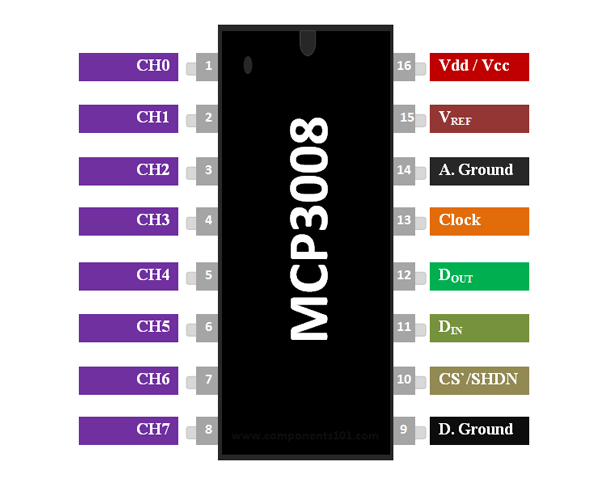
\includegraphics[width=0.6\columnwidth]{Figures/MCP3008Pinout}
\caption{The pinout of the MCP3008}
% \label{}
\end{figure}

\subsection{Walkthrough}
\begin{enumerate}
    \item Enable SPI using the raspi-config tool
    \item Install the MCP3008 Adafruit library
    \begin{lstlisting}[gobble=4]
    $ sudo apt-get update
    $ sudo apt install build-essential python3-dev python3-smbus python3-pip
    $ sudo pip3 install adafruit-circuitpython-mcp3xxx
    \end{lstlisting}
    \item Build the circuit described above.
    \item Create a new python file
    \item Place the following code in it:
    \begin{lstlisting} [gobble=4]
    import busio
    import digitalio
    import board
    import adafruit_mcp3xxx.mcp3008 as MCP
    from adafruit_mcp3xxx.analog_in import AnalogIn

    # create the spi bus
    spi = busio.SPI(clock=board.SCK, MISO=board.MISO, MOSI=board.MOSI)

    # create the cs (chip select)
    cs = digitalio.DigitalInOut(board.D5)

    # create the mcp object
    mcp = MCP.MCP3008(spi, cs)

    # create an analog input channel on pin 0
    chan = AnalogIn(mcp, MCP.P0)

    print('Raw ADC Value: ', chan.value)
    print('ADC Voltage: ' + str(chan.voltage) + 'V')
    \end{lstlisting}
    If you run this code you will see the reading from the LDR. Cover the sensor and run the code again. The reading should change.
    \item Adapt your code to read from both sensors and print to terminal every ten seconds. You \textbf{must} use a thread. You can read about simple threading in Python \href{http://wiki.ee.uct.ac.za/RaspberryPi:ProgrammingInPython}{here}. The output of your application should look as follows:
    \begin{lstlisting}[gobble=4]
    Runtime     Temp Reading    Temp	
    0s          <ADC value>	    <converted temp>  C
    10s         <ADC value>	    <converted temp>  C
    20s         <ADC value>	    <converted temp>  C
    30s         <ADC value>	    <converted temp>  C
    40s         <ADC value>	    <converted temp>  C
    50s         <ADC value>	    <converted temp>  C
    60s         <ADC value>	    <converted temp>  C
    \end{lstlisting}
    \item Runtime must be calculated, and not be implemented as a counter
    \item Add a button to toggle the rate of sampling between 10s, 5s and 1s
\end{enumerate}

\subsection{Requirements for submission}
\label{prac4sub}
There are two items you need to uploaded to Vula for submission of this practical assignment: 
\begin{enumerate}
    \item Your prac report provided as a single PDF file, named \verb|Prac5_<studnum1>_<studnum2>.pdf|
    \item A short demo video in which you present your design and implementation (see demo marking guide in Table \ref{tbl:Prac5DemoValidation} below).
\end{enumerate}


\textbf{Report Requirements}

The report should contain the following:
\begin{enumerate}
    \item The circuit diagram you used
    \item A paragraph on your validation and testing for the values you got from the ADC for both light and temperature
    \item Your Python code (screenshots of code will not be marked)
\end{enumerate}
Marks will be awarded for:
\begin{itemize}
    \item Neatness (circuit diagram and code)
    \item Correctness
    \item Using threads correctly
    \item Correct implementation of the temperature reading algorithm
\end{itemize}

\textbf{Demo Marking Guide}

Marks will be deducted for:
\begin{itemize}
    \item Not following instructions
    \item Plagiarism/Copying
\end{itemize}

You can prepare a short video, about 5 minutes will probably be sufficient. There is no minimum duration, but you need to respond to the aspects as listed in the marksheet below; but we do \textit{not} want videos beyond 10 minutes in length. The demo should respond to the following aspects (the marking allocations are shown on the right):

\label{sec:ProjAValidation}
\begin{table}[H]
\caption{The Mark sheet for the demo aspect of Prac5}
\label{tbl:Prac5DemoValidation}
\centering
\resizebox{\textwidth}{!}{%
\begin{tabular}{|l|l|l|r|c|}
\hline
% \multicolumn{3}{|l|}{{\ul \textbf{Project Validation Sheet}}}  & \multicolumn{2}{l|}{\begin{tabular}[c]{@{}l@{}}\textbf{Marked by:} \\ \\\end{tabular}} \\ \hline
% \multicolumn{7}{|l|}{\begin{tabular}[c]{@{}l@{}}\textbf{Student Numbers:} \\ \\ \\\end{tabular}} \\ \hline
\textbf{Category} & \textbf{Item} & \textbf{Description} & \multicolumn{1}{c|}{Max Mark} & \begin{tabular}[c]{@{}c@{}}Attempt\\ 1\end{tabular} \\ \hline 

\textbf{Intro} & \begin{tabular}[c]{@{}l@{}}Intro \\ and division of \\ workload \end{tabular} & \begin{tabular}[c]{@{}l@{}}Start off the demo by\\ indicating your prac team \\ members. \\ Indicate how you \\ divided up the work \end{tabular} & 6 &    \\ \hline

\textbf{Design} & Design and connections & \begin{tabular}[c]{@{}l@{}}Indicate the way\\ you hooked up the ADC \\ (using a circuit diagram or alternate \\ clear visualization) \\ and present the software design \\ e.g block diagram or flow chart \\ of your program \end{tabular} & 5 &  \\ \hline
 &  & \begin{tabular}[c]{@{}l@{}}Point to significant parts of \\ your code that \\ concerns the hardware and \\ any timing aspects \\ (use of comments,\\ and reminders in the \\ code, e.g. of things to draw \\ attention to in the demo are recommended)\end{tabular} & 5 &  \\ \hline
 
ADC Test & Testing Implementation & \begin{tabular}[c]{@{}l@{}}Run through the \\ operation of your \\ prototype  (e.g. increase light \\ decrease light, etc) \end{tabular} & 10 &  \\ \hline

%  & Potentiometer & \begin{tabular}[c]{@{}l@{}}Responds to changes input, \\ reading displayed is between\\ 0 and 3.3V\end{tabular} & 2 &  &  &  \\ \hline
Conclude & Conclude the presentation & \begin{tabular}[c]{@{}l@{}}Report on the extent the test was \\ successful provide some suggestions \\ for how you might improve \\ things or add features if time allowed \end{tabular} & 4 & \begin{tabular}[c]{@{}l@{}} \end{tabular}  \\ \hline
Mark &  &  & 30 & \begin{tabular}[c]{@{}l@{}} \\ \\\end{tabular} \\ \hline
\end{tabular}%
}
\end{table}



% % PART A - SPI sensor reading, MQTT
% Part B - Geographic Information System with MQTT data?
\newpage
\begin{center}
    \rule{\linewidth}{0.2 mm} \\[0.4 cm]
	{ \huge \bfseries Mini-Projects A \& B}\\
	\huge Terrarium Logger
	\rule{\linewidth}{0.2 mm} \\[1.5 cm]
	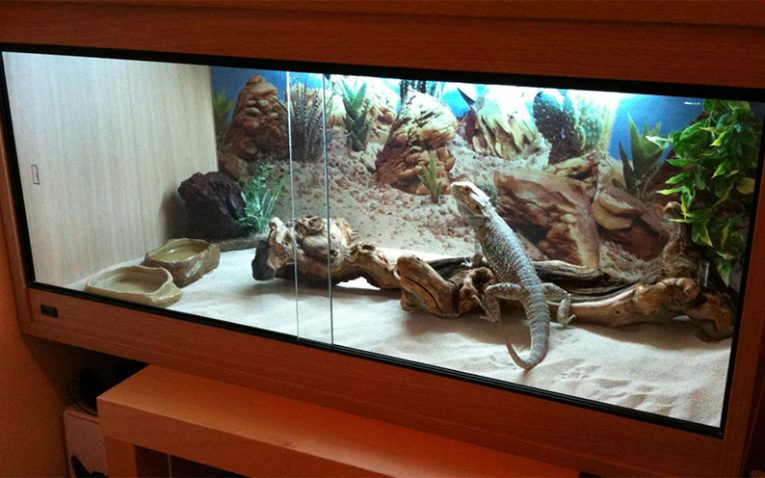
\includegraphics[scale = 0.5]{Figures/terrarium.jpg}\\[1 cm]
	\textsc{\Large EEE3096S}\\[0.5 cm]
	\textsc{\large Embedded Systems II}\\[0.5 cm]
	\textsc{\LARGE University of Cape Town}\\[0.5 cm]
\end{center}
\newpage
\chapter{The Terrarium Mini-logger}
\section{Overview}
The mini-project is a chance for you to use what you have learnt in this course and test your problem-solving skills. The projects use everything learnt in the previous practicals - so here's to hoping that you paid attention and remembered those! All students need to do Mini-Project A. Only CS students (EEE3095S students) need to do Mini-Project B.

\subsection{Scenario}
Your uncle has heard of you achieving great things in an embedded systems course at university. He approaches you and requests your assistance in building an environment logger for his terrarium to assist with taking care of his pet bearded dragon. As they are ridiculously adorable (bearded dragons, not uncles) - you agree to assist.

\begin{figure}[H]
\centering

\includegraphics[width=0.7\columnwidth]{Figures/uncledragon.png}
\caption{You can read more about this adorable creature \href{https://knowyourmeme.com/memes/butter-the-bearded-dragon}{here}}
\label{ButterDragon}
\end{figure}

Your uncle needs to monitor temperature and light levels at varying intervals, which needs to be adjusted by a button press. He also wants to enable and disable logging by pressing a second button. Your uncle has a spare system which they can use to log into the Pi remotely and monitor console output, which he lists as one of the requirements. However, they wish to also monitor the terrarium remotely when they are not there. Their son, who plays with Arduinos, has spoken a lot about \href{https://blynk.io/}{Blynk} for IoT devices. You decide to look into these options for remote monitoring. 

The following requests were also made:
\begin{itemize}
    \item the most recent 20 samples are stored on an EEPROM chip as backup, in the case that internet access is lost.
\end{itemize}


\subsection{Basic Details}
Your objective for Mini-Project A environment logger. Mini-Project B is an add-on to Mini-Project A which involves minimal work to extend the functionality of the monitoring system. If you are in a group with both CS and EE members, you can both work together on Mini-Project A. For Mini-Project B, CS students can chose to work alone or partner up with another CS student to form new groups of 2.

Generally speaking, an environment logger interacts with the world around it by measuring various factors from GPS location to air pollution. While a single sensor is useful to monitor a single location, many can be scattered around a broader area to monitor that area as well as any patterns emerging in that broader area. This data can be used to track changes over time to forecast effects or make inferences between locations and how they might affect each other. In these mini-projects there is not much data to track and there aren't many potential effects to forecast, though the principles remains the same.

Project A and B differ in how that data is presented to end users. Project A is simply accessed through a terminal. Project B will add reporting data to Blynk, an app that can be installed on smartphones. The environment logger can also be controlled via the Blynk app.

\textbf{NOTE: FOR EACH SUBMISSION, BOTH STUDENTS NEED TO INCLUDE A SIGNED PLAGIARISM DECLARATION AT THE END OF THE SUBMISSION, WITH THE SUBMISSION AND BOTH PLAGIARISM DECLARATIONS IN A SINGLE PDF. THE FORM CAN BE FOUND AT THE END OF THIS MANUAL.}

\chapter{Mini-Project A}
\label{sec:ProjA}
This project examines ELO5.2, which requires the student to develop a representative embedded system. It requires hardware/software interfacing, so an ADC is sampled by software, and processing operations are applied to read the data. 

\section{Project Requirements}
The Project is split into Milestones in order to help you plan time and ensure you aren't overburdened with work a few days before the final deadline. Dates for submission will be put on Vula. The milestones are as follows:
\begin{enumerate}
    \renewcommand{\theenumi}{\Alph{enumi}}
    \item Planning and System Design\\
    For this milestone we expect to see the following:
    \begin{itemize}
        \item A Gantt Chart indicating your planned activities with the project
        \item A circuit diagram for the system
        \item A choice on how you plan to approach the project (e.g. Spiral, waterfall, etc.) as well as a justification as why
        \item A flowchart detailing how the system operates
    \end{itemize}
    \item Code and Report\\
    The final hand in will be the report and your code submission. Details on these can be found in the marking guides.
\end{enumerate}

\section{Outcomes}
In addition to creating a working system, you will learn about the following in this project:
\begin{itemize}
    \item Technical outcomes
    \begin{itemize}
        \item ADC - \href{https://cdn-shop.adafruit.com/datasheets/MCP3008.pdf}{MCP3008}
        \item Temperature sensor - \href{http://ww1.microchip.com/downloads/en/devicedoc/20001942g.pdf}{MCP9700A}
        
    \end{itemize}
    \item Other outcomes
    \begin{itemize}
        \item Team Work
        \item Design methodologies, such as the Waterfall, Spiral and V Models.
        \item Planning and time management
    \end{itemize}
    
    
\end{itemize}

\section{Deliverables}
At the end of this project, you must:
\begin{itemize}
    \item Submit all milestones
    \item For information on the marks and what sections to cover, refer to the marking guide in Section \ref{sec:ProjAMarks}
\end{itemize}

\section{System Overview}
Figure \ref{fig:SystemOverview} shows the system overview for the mini-project.
\begin{figure}[H]
\centering
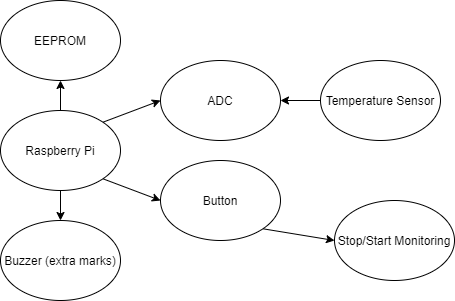
\includegraphics[width=0.6\columnwidth]{Figures/2020-SystemOverview-A}
\caption{Components of Mini-Project A}
\label{fig:SystemOverview}
\end{figure}

\section{Hardware requirements}
You will need to build your designed circuit on a breadboard and demonstrate it in the video you create.

\section{Software requirements}
You need to do the following:
\begin{itemize}
    \item Set up the EEPROM. 
    \item Create a thread for reading from the ADC. The value read from the temperature sensor needs to be converted to degrees Celsius. See the datasheet (linked above) for the formula.
    \item Create interrupts for all the button functionality (don't forget to debounce your inputs)
    \item Create an output signal to trigger the buzzer (bonus marks)
    \item In the main() loop, print values to the screen as described in Section \ref{sec:ProjDescription}
\end{itemize}

\section{Description}
\label{sec:ProjDescription}
\begin{itemize}
    \item By default, the system continuously monitors the sensors every 5s using this format:
    \begin{table}[H]
    \centering
    \begin{tabular}{|l|l|l|l|}
    \hline
    Time     & Sys Timer & Temp  &  Buzzer  \\ \hline
    10:17:15 & 00:00:00  & 25 C  & *        \\ \hline
    10:17:20 & 00:00:05  & 25 C  &          \\ \hline
    10:17:25 & 00:00:10  & 25 C  &          \\ \hline
    10:17:30 & 00:00:15  & 25 C  &          \\ \hline
    10:17:35 & 00:00:20  & 25 C  &          \\ \hline
    10:17:35 & 00:00:20  & 25 C  & *        \\ \hline
    \end{tabular}
    \end{table}
    \item The stop switch stops or starts the monitoring of the sensors. The system timer is not affected by this functionality. The screen must also be cleared when logging is stopped, and a message printed to display to inform the user that the logging has stopped.
\end{itemize}

\section{Marking Guide}
\label{sec:ProjAMarks}
\begin{longtable}[c]{|l|l|}
\caption{Project A marking Guide}
\label{tbl:ProjAMarks}
\\\hline
\textbf{Heading} & \textbf{Report} \\ \hline
\endfirsthead
%
\endhead
%
Introduction & \begin{tabular}[c]{@{}l@{}}Provide a short introduction ($\sim \frac{1}{2}$ page) to your project explaining your main\\ design choices and how the report has been structured \textbf{{[}15 marks{]}}\end{tabular} \\ \hline
Requirements & \begin{tabular}[c]{@{}l@{}}The requirements section should provide a refined UML Use Case\\ diagram of the system, according to your implementation, and any\\ accompanying text that is needed to clarify the requirements.\\ Highlight any departures or additions that you may have made compared to\\ the original project description given in this document. \textbf{{[}15 marks{]}}\end{tabular}  \\ \hline
\begin{tabular}[c]{@{}l@{}}Specification \\ and Design\end{tabular} & \begin{tabular}[c]{@{}l@{}}This section should provide a UML State Chart describing the main\\ operation. Add a UML class or deployment diagram (or other suitable\\ diagram) to indicate the structuring of your implementation (e.g. code\\ modules/classes you may be using). You don’t need to provide fine detail of\\ the system, the diagram(s) can be e.g. at the level of functions. You should\\also include a circuit diagram \textbf{{[}20 marks{]}}\end{tabular}  \\ \hline
Implementation & \begin{tabular}[c]{@{}l@{}}This section should give some snippets of important code and explanations for\\ this (or referring to particular functions in code files). The point here\\ is elaborating any parts of the State Chart that are not so straightforward\\ to turn into code. \textbf{{[}20 marks{]}}\end{tabular} \\ \hline
\begin{tabular}[c]{@{}l@{}}Validation and\\ Performance\end{tabular} & \begin{tabular}[c]{@{}l@{}}Provide at least a paragraph or two explaining the performance of the\\ system. A snapshot could be included and you could show test cases where\\ you have tested that the system works reliably (e.g. using a powersupply to set \\ the value given to the ADC). \textbf{{[}20} \textbf{marks{]}}\end{tabular} \\ \hline
Conclusion & \begin{tabular}[c]{@{}l@{}}Give a summary of the extent that the system was found to be successful.\\ Discuss if you think that a system working in this way might be\\ considered a potentially useful product. \textbf{{[}10 marks{]}}\end{tabular}  \\ \hline
References & Provide a few references if relevant.  \\ \hline
Total & 100 \\ \hline
\end{longtable}
\chapter{Mini-Project B}
This project is for CS students only.\\

\section{Scenario}
Your uncle appreciates the work you have done developing a rough prototype. Because you did such a good job of developing the base system, your uncle has asked you to develop a means of a system where they can access their data remotely. You decide to do this as simply as possible, making use of an application called \href{https://blynk.io/}{Blynk}.



\subsection{Overview}
Essentially, this is a repeat of the first project, but adds a button to change the interval reading and makes the data accessible through Blynk.

\subsection{Deliverables}
At the end of this practical, you must
\begin{itemize}
    \item Submit a short write up. See the marking guide in section \ref{sec:ProjBMarks}
\end{itemize}

\subsection{Hardware Required}
The hardware from mini-project A and an additional button.

\subsubsection{Software Requirements}
\begin{itemize}
    \item You need to add Blynk.
    \item You need to add functionality for changing the reading interval between 2, 5 and 10 seconds.
\end{itemize}

\begin{multicols}{2}
Figure \ref{fig:blynkexample} shows an example of what the app you create in Blynk might look like. This is the example from last year's project, but you can see there's a terminal for accessing the output of the print statements and a space for values as read from the ADC. Last year's project also had an alarm, which is not a feature in this year's project so you need not include one. There are various widgets in Blynk. It's suggested you play with your energy budget to develop the most intuitive and aesthetically pleasing design possible.
\vfill\null
\columnbreak
\begin{figure}[H]
\centering
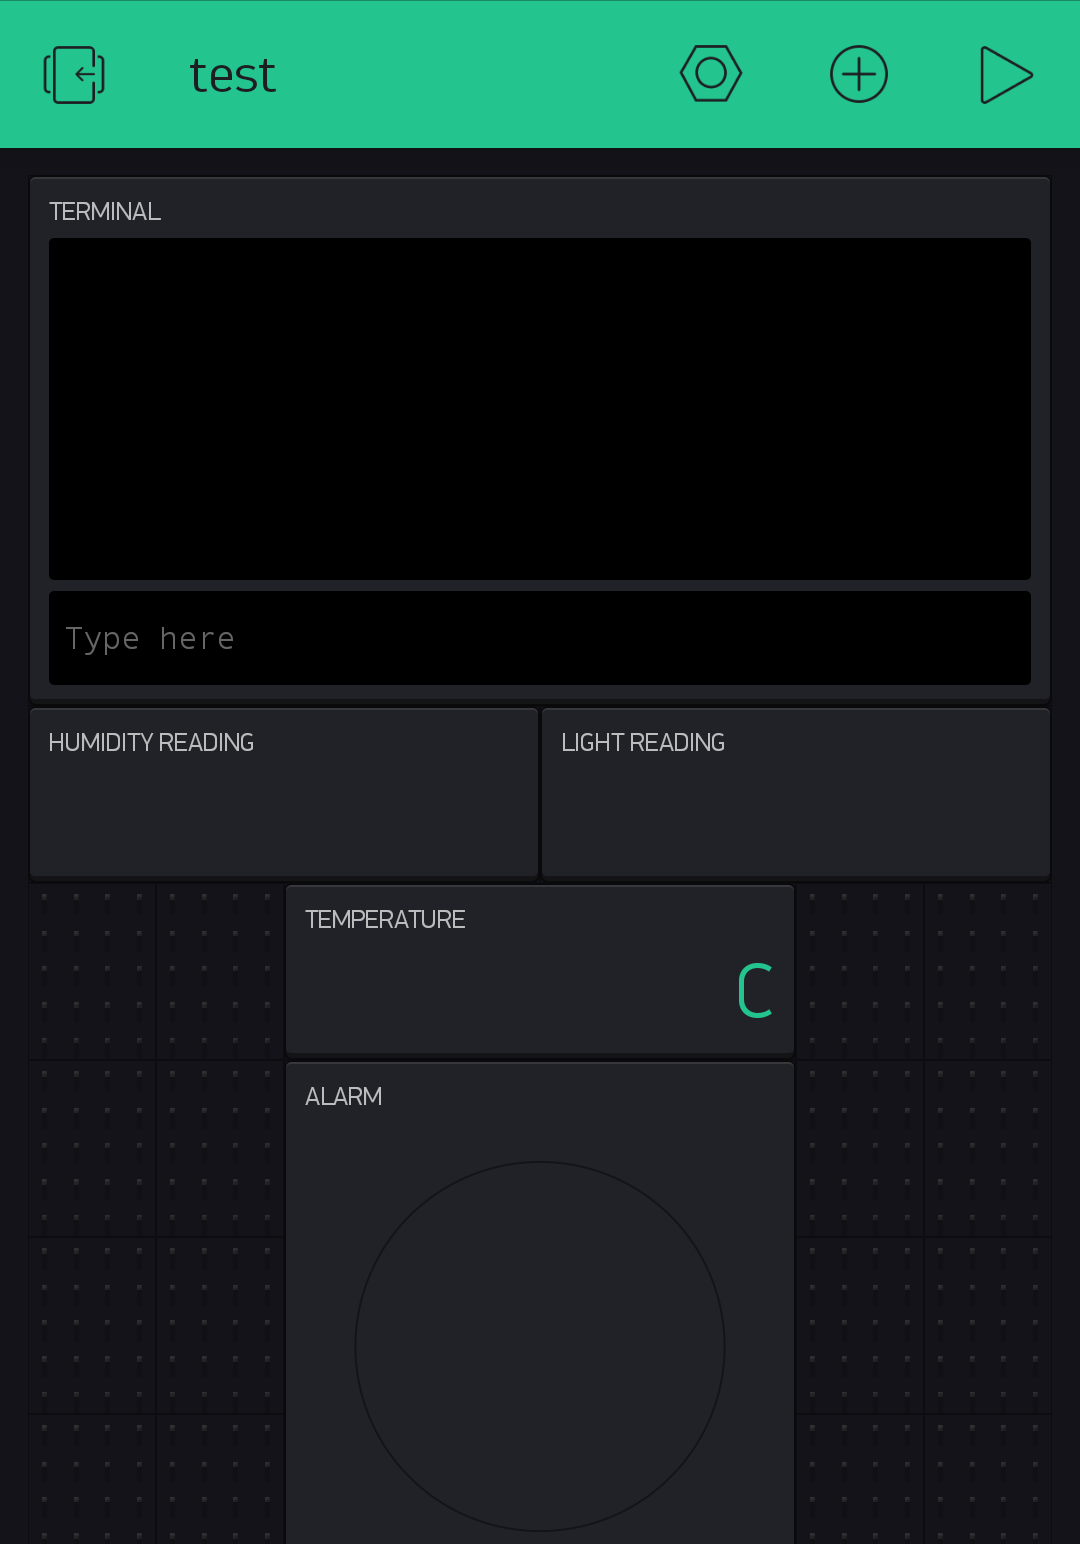
\includegraphics[width=0.75\columnwidth]{Figures/blynkexample}
\caption{Example Blynk Project}
\label{fig:blynkexample}
\end{figure}
\end{multicols}

\subsection{Marking Guide}
\label{sec:ProjBMarks}
\begin{table}[H]
\centering
\caption{The Write Up Format For mini-project B}
\label{tbl:ProjBMarks}
\begin{tabular}{|l|l|l|}
\hline
\textbf{Section of Report} & \textbf{Description} & \textbf{Marks} \\ \hline
\textbf{Introduction} & An introduction to what's new in this project & 10 \\ \hline
\textbf{Design} & \begin{tabular}[c]{@{}l@{}}Design of the system. Design of the server. \\ Talk about the stack used for development. \\ Include UML and block diagrams, and \\ mention any hardware/software\\ interfacing issues.\end{tabular} & 30 \\ \hline
\textbf{\begin{tabular}[c]{@{}l@{}}Implementation/\\ Build Proces\end{tabular}} & \begin{tabular}[c]{@{}l@{}}Some code snippets and steps in building \\ the device and server.Can think of this as a\\ simple methodology.\end{tabular} & 15 \\ \hline
\textbf{Instructions for use} & \begin{tabular}[c]{@{}l@{}}How to operate the system. You should \\ include some screenshots and photos.\end{tabular} & 15 \\ \hline
\textbf{Testing/Results} & \begin{tabular}[c]{@{}l@{}}How did you ensure your system works? \\ What did you do to test the functionality, \\ and what were the results? You can include\\ screenshots or photos, but you need to talk \\ about them (it's not enough to just have a \\ photo).\end{tabular} & 20 \\ \hline
\textbf{Conclusions} & \begin{tabular}[c]{@{}l@{}}How well did your system work? Did you \\ achieve the objectives? What could you do \\ to improve the system?\end{tabular} & 10 \\ \hline
\textbf{TOTAL} &  & \textbf{100} \\ \hline
\end{tabular}%
\end{table}


\chapter{Acknowledgements}
\begin{enumerate}
    \item Image use \href{https://onlineplantsindubai.weebly.com/uploads/1/0/9/0/109064913/air-plants-terrarium-as-bearded-dragon-terrarium_1_orig.jpg}{onlineplantsindubai.weebly.com}
    \item The meme template used in Figure \ref{ButterDragon} is of Butter the bearded dragon, which is accessible through a Google search
\end{enumerate}

\newpage

\textbf{Declaration of non-plagiarism}

\begin{itemize}
    \item I know that plagiarism is wrong. Plagiarism is to use another’s work and pretend that it is one’s own.
    \item I have used the \rule{4cm}{1pt} convention for citation and referencing. Each contribution to, and quotation in, this essay/report/project/submission from the work(s) of other people has been attributed, and has been cited and referenced.
    \item This essay/report/project/submission is my own work.

    \item I have not allowed, and will not allow, anyone to copy my work with the intention of passing it off as his or her own work. 

\end{itemize}

 

Name \rule{4cm}{1pt}  Student Number \rule{4cm}{1pt}

 

Signature \rule{4cm}{1pt}     Date \rule{4cm}{1pt}

 






\end{sloppypar}
\end{document}
